%author: Simone Notargiacomo, Lorenzo Tavernese, Ibrahim Khalili
%date: 21 Settembre 2008
\documentclass[a4paper,12pt,oneside]{report}
\usepackage[hyperindex]{hyperref}
\usepackage[utf8]{inputenc}
\usepackage[italian]{babel}
\usepackage[T1]{fontenc}
\usepackage{makeidx}
\usepackage{graphicx}
\usepackage{fancyhdr}
\usepackage{subfigure}
\usepackage{amssymb}
\usepackage[reqno]{amsmath}
\usepackage{amsfonts}
\usepackage{natbib}
\usepackage{latexsym}
\usepackage{float}
\usepackage{listings}
\usepackage[usenames,dvips]{color}
\usepackage{multicol}
\usepackage{framed}

\linespread{1.3}
\makeindex
\lstset{language=Java}
\lstset{frameround=fttt}
\lstset{basicstyle=\scriptsize}
\lstset{stringstyle=\ttfamily}
\lstset{showstringspaces=false}
\lstset{morecomment=[s]{/*}{*/}}
\lstset{morecomment=[n]{/*}{*/}}
\lstset{morekeywords={Context, SLAContract, Notify, Agent, String, AID, Float, Hashtable, LinkedList, Queue, Enumeration, SLARequesterBehaviour, SLAReqReceiverBehaviour, ContextProducerBehaviour, ViolationConsumerBehaviour, RmConsumerBehaviour, ContextManagerAgent, CpuResourceBehaviour, RamResourceBehaviour, MemoryResourceBehaviour, EnergyResourceBehaviour, LatencyResourceBehaviour, ReliabilityResourceBehaviour, ReqIntervalResourceBehaviour, RamRmAgent, MemoryRmAgent, EnergyRmAgent, CpuRmAgent, LatencyRmAgent, ReliabilityRmAgent, ReqIntervalRmAgent, AgentLauncher, SLAReceiverBehaviour, SLACheckerBehaviour, SLAStarterBehaviour, ContextConsumerBehaviour, MigrationUtil, SLACheckerAgent, ReqIntervalBehaviour, NotifyReceiverBehaviour, LatencyBehaviour, RamBehaviour, CpuBehaviour, MemoryBehaviour, EnergyBehaviour, ReliabilityBehaviour, CpuAgent, ResourceAgent, MemoryAgent, EnergyAgent, ReliabilityAgent, ReqIntervalAgent, LatencyAgent, RamAgent, DFUtil, Context, Notify, SLAContract, DataWriter, PropertiesReader, DsmServerBehaviour, DsmDataManager, Tuple, DsmServerAgent, DsmClient}}
\lstset{aboveskip=\bigskipamount}
\lstset{belowskip=\bigskipamount}
\lstset{showlines=false}
\lstset{breaklines=true}
\definecolor{light-gray}{gray}{0.95}
\lstset{backgroundcolor=\color{light-gray}}
\lstset{frame=trBL}

\newcommand{\code}[1]{%
	\texttt{#1}\index{#1}
}%
\newcommand{\var}[1]{%
	\emph{#1}\index{#1}%
}%

\definecolor{lightgray}{gray}{0.95}
\newcommand{\sfondo}
{
	\AddToShipoutPicture{
		\AtTextCenter{
			\put(0,-5){
				\makebox(0,0)[c]{
					\resizebox{2.2\textwidth}{!}{
						\rotatebox{60}{
							\textsf{\textbf{\textcolor{lightgray}{TaskSpider}}}
						}
					}
				}
			}
		}
	}
}

\begin{document}
\begin{titlepage}
\begin{center}
\LARGE{Università degli Studi di Roma Tor Vergata}\\
\vspace{10mm}
%\begin{center}

\includegraphics[scale=0.50]{etc/logo.jpg}\\
%\end{center}
Facoltà di Ingegneria\\
\vspace{5mm}
\normalsize{Corso di Informatica Mobile}\\
\vspace{20mm}

\includegraphics[scale=0.60]{etc/slash.jpg}\\
%\large{}\\
%\\url{http://mislash.googlecode.com}\\
\end{center}
\vspace{40mm}
\begin{minipage}[t]{0.30\textwidth}
\begin{center}
{\normalsize{Professore:\\
Vincenzo Grassi}}
\end{center}
\end{minipage}
\hfill
\begin{minipage}[t]{0.30\textwidth}
\begin{center}
{\normalsize{Studenti:\\
Simone Notargiacomo\\
Lorenzo Tavernese\\
Ibrahim Khalili}}
\end{center}
\end{minipage}
\vspace{10mm}
\begin{center}
Anno Accademico 2007-2008
\end{center}

\end{titlepage}
\pagebreak
\pagestyle{fancy}
\fancyhead[RO]{}
\fancyhead[LO]{\slshape \leftmark}
\fancyfoot[C]{\thepage}
\renewcommand{\headrulewidth}{0.4pt}
\oddsidemargin 0.6in
%\renewcommand{\footrulewidth}{0.4pt}
\setcounter{page}{1}
\pagenumbering{roman}
\tableofcontents

\chapter*{Abstract}
\addcontentsline{toc}{chapter}{Abstract}
Nel mondo dell'Informatica si è diffuso da molto tempo il bisogno di sviluppare applicazioni per dispositivi mobili, quali notebook, smartphone, tablet ed altro ancora; in particolare si è raggiunta la necessità di sviluppare applicazioni distribuite per dispositivi mobili, ovvero il \var{Mobile Computing}. Grazie a questo bisogno sono nate molte nuove tecniche che hanno apportato migliorie alla comunicazione tra dispositivi, come la stipulazione di \var{SLA} (Service Level Agreement: Contratti basati sul livello di servizio) tra richiedenti e fornitori di servizi, ed infine le \var{dsm} (Distribuited Shared Memory). Durante il corso di Informatica Mobile è stato richiesto di realizzare un sistema che simulasse il comportamento di alcuni richiedenti e fornitori dopo aver stipulato un contratto sulla qualità del servizio, sfruttando \var{dsm} per la comunicazione dei dati. In questa relazione verranno trattate le problematiche incontrate nella progettazione del sistema, ed in particolare tutte le scelte implementative effettuate, nonchè i modelli matematici ed empirici. Inoltre verranno presentati anche dei test di esecuzione con i relativi dati sulle performance; infine si riporteranno le conclusioni a cui si è giunti ed i possibili sviluppi futuri.
\setcounter{page}{1}
\pagenumbering{arabic}
\chapter{Introduzione}\label{cap:introduzione}
Per comprendere a fondo l'entità di tale progetto si riportano di seguito le specifiche del progetto, in quanto consente al lettore di entrare nell'ottica del problema, inoltre si fornirà una breve panoramica relativa al paradigma DSM, agli agenti mobili e al framework JADE.
\section{Specifiche problema}
\subsection{Logica applicazione}
Si richiede di progettare una architettura di supporto al monitoraggio e controllo di SLA\cite{gino} in ambiente (possibilmente) mobile. L’architettura del servizio è basata sulla definizione di un certo numero di componenti “logici”: SLA Checker (SC), Context Manager (CM), Resource Monitor (RM). Tali entità interagiscono tra loro unicamente tramite il meccanismo DSM ("tuple space"). Il ruolo di tali entità viene descritto come segue:
\begin{description}
\item[SLAchecker (SC):] data una coppia fornitore/richiedente servizio, che ha stipulato un SLA, SC ha il compito di controllare il rispetto dei parametri del contratto sia da parte del fornitore che del richiedente, e segnalare eventuali violazioni ad entrambi. A questo scopo, SC raccoglie informazioni fornite da opportuni componenti di tipo Monitor presenti sia sul nodo del fornitore che del richiedente, relative a (per esempio):
\begin{itemize}
\item tempo di risposta osservato per una richiesta;
\item affidabilità (completamento con successo) di una richiesta;
\item intervallo di tempo tra due richieste consecutive.
\end{itemize}
I dati “grezzi” ricevuti dai componenti di monitoraggio vengono elaborati da SC per calcolare i valori degli indici di interesse.
\item[Context Manager (CM):] è un componente associato a un particolare nodo di elaborazione e il suo ruolo è quello di fornire informazioni su vari tipi parametri che caratterizzano il contesto di esecuzione di componenti presenti su quel nodo, p.es.:
\begin{itemize}
\item utilizzazione cpu;
\item RAM disponibile;
\item memoria stabile (disco, o altro) disponibile;
\item tipo di rete e banda disponibile;
\item energia disponibile.
\end{itemize}
\item[Resource Monitor (RM):] un componente di questo tipo fornisce le informazioni relative a una delle risorse elencate sopra.
\end{description}
\subsection{Ambiente d'uso}
L’ambiente in cui si immagina che il servizio di controllo di SLA venga realizzato è costituito, in generale, da una molteplicità di nodi (fissi o mobili) con vari livelli di disponibilità di risorse interne (memoria, cpu, ecc.), connessi tra loro da infrastrutture di comunicazione di varia qualità. Su tali nodi sono in esecuzione componenti che offrono/richiedono servizi. Ogni volta che una coppia fornitore/richiedente stipula un SLA, il controllo di questo SLA viene affidato a un componente SC.
\subsection{Lavoro progettuale}
Si richiede di progettare e realizzare, utilizzando la piattaforma JADE (\url{http://jade.tilab.com}), l’architettura indicata nella sezione precedente. In particolare, occorre definire una localizzazione dei componenti e organizzazione del modello DSM (basato sulla realizzazione di uno o più "tuple space") che sia adeguata alla esecuzione del servizio di controllo SLA in un ambiente possibilmente mobile, caratterizzato da possibile scarsità di risorse per i componenti in esecuzione su determinati nodi. Il livello di adeguatezza andrà valutato rispetto alla capacità di ottimizzare misure di prestazione quali:
\begin{itemize}
\item traffico generato su rete;
\item consumo di energia da parte di nodi mobili;
\item carico computazionale/di memorizzazione per nodi mobili;
\end{itemize}
tenendo anche conto del fatto che il contesto (disponibilità di risorse) in cui opera il servizio di controllo SLA può variare nel tempo, per esempio per effetto della mobilità di alcuni nodi.
\section{Distributed Shared Memory}
Il paradigma DSM fornisce agli host in un sistema distribuito la vista di uno spazio comune condiviso attraverso spazi di indirizzamento disgiunti, in cui la sincronizzazione e la comunicazione fra i partecipanti avvengono tramite operazioni sui dati comuni. La nozione di \var{tuple space} è stato originariamente integrato in Linda, e fornisce una semplice e potente astrazione per accedere alla memoria condivisa. Un \var{tuple space} è composto di una collezione di tuple ordinate, accessibili in egual modo da tutti gli host del sistema distribuito. La comunicazione tra hosts avviene tramite l'inserimento/rimozione di tuple nel/da \var{tuple space}. Possono essere eseguite tre operazioni di base: \var{out()} per esportare una tupla nel \var{tuple space}, \var{in()} per importare (e rimuovere) una tupla e \var{read()} per leggere, senza rimuovere, una tupla. Il modello di interazione offre disaccoppiamento sia spaziale che temporale, pochè consumatore e produttore non hanno bisogno di conoscersi e il creatore di una tupla non ha bisogno di sapere l'uso che verrà fatto di tale tupla. Nonostante tutto, non si ha un disaccoppiamento da un punto di vista della sincronizzazione dal lato del consumatore.
\begin{figure}[H]
\begin{center}
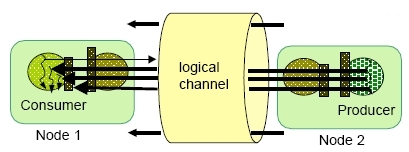
\includegraphics[scale=0.7]{etc/dsm1.jpg}
\caption{DSM}
\label{dsm}
\end{center}
\end{figure} 

\section{Mobile Agent}
Un agente mobile è un componente software in grado di traserirsi su nodi remoti di una rete e di interagire con le risorse nei nodi visitati, scoprendo i servizi offerti.
Dalla definizione fornita si arguisce che l'Agente deve possedere un certo grado di \var{intelligenza}, sia per le decisioni che deve prendere una volta spedito, sia per la capacità di memorizzare i risultati ottenuti su ciascun nodo (capacità di mantenere ed aggiornare il suo stato).
La possibilità per un agente di muoversi e di conseguenza il comportamento che questo può assumere si deve basare sugli obiettivi definiti nel suo stato. Tale concetto di mobilità unito a quello di agente ha permesso di conferire a questo componente la capacità di cooperare al fine di poter risolvere un dato problema.
Il processo di trasferimento del codice e del relativo stato può avvenire secondo due modalità differenti:
\begin{itemize}
\item Clonazione: il codice e lo stato vengono duplicati nel nodo di arrivo senza rimuoverli nel nodo di partenza
\item Migrazione: il codice e lo stato vengono copiati nel nuovo nodo e rimossi dal vecchio. 
\end{itemize}
Terminato il processo di migrazione l'agente deve essere in grado di interagire con le risorse locali al fine di usufruire dei servizi offerti dal nodo ospite.
Il meccanismo di interazione con le varie risorse presenti viene facilitato grazie all'utilizzo della tecnologia ad oggetti, al contrario del procedimento di \var{discovery} dei servizi, il quale prevede un modello di  \var{introspezione}  degli oggetti, che mantenga le informazioni accessibili dinamicamente.
Si può quindi intuire che se da un punto di vista teorico si ha grande convenienza nell’utilizzo di Agenti, in pratica non sempre risulta possibile usufruire di tali vantaggi. E’ importante evitare di cadere nella tentazione assolutista con la quale si cerca di applicare una tecnologia in ogni possibile dominio o circostanza. Possiamo sicuramente affermare che la soluzione ad Agenti può essere più conveniente rispetto ad altri approcci a seconda di circostanze quali domini, infrastrutture di rete, compatibilità con altre
tecnologie di contorno.  

\section{JADE}
JADE è un framework interamente realizzato in Java, che permette di  semplificare l'implementazione di \var{Multi Agent Systems} (MAS),associando diversi container agli agenti, i quali hanno la possibiltà di comunicare sulla stessa o su piattaforme differenti.
I vari containers possono essere raggruppati formando così una \var{platform}.
\begin{figure}[H]
\begin{center}
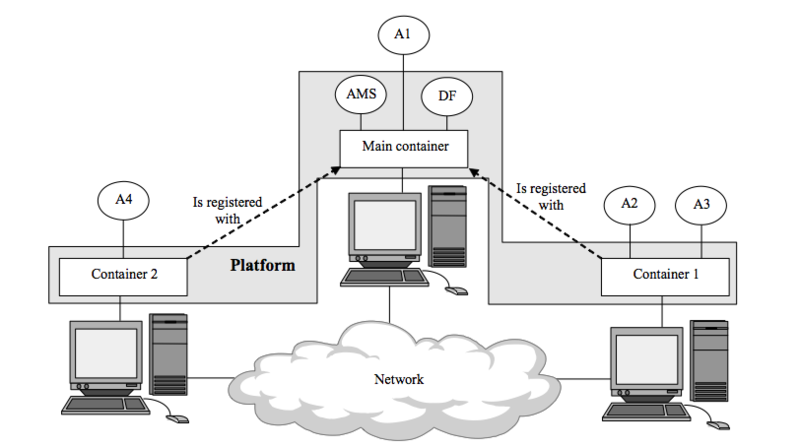
\includegraphics[scale=0.5]{etc/jade_architettura.png}
\caption{architettua di JADE}
\label{architettura_jade}
\end{center}
\end{figure} 
Ogni platform deve avere un \var{Main Container}, il quale possiede due agenti specializzati chiamati rispettivamente \var{AMS agent} e \var{DF agent}:
\begin{itemize}
\item L'\var{AMS} (Agent Management System) ha il compito di svolgere la funzione di supervisore controllando l’accesso e l’uso della
piattaforma da parte degli agenti.Inoltre mantiene un registro degli identificatori degli agenti (AID) e del loro stato, in quanto ogni agente
 è obbligato a registrarsi per ottenere un AID valido . 
\item Il \var{DF} (Directory Facilitator) ha il compito di implementare un servizio di pagine gialle che pubblicizza i servizi degli agenti della piattaforma in modo che altri agenti che richiedono tali servizi possono trovarli.
\end{itemize}
Le varie operazioni che gli agenti sono in grado di compiere vengono definite attaverso oggetti di tipo \var{Behaviour}, i quali forniscono l'implementazione dei task rischiesti.Esistono diversi tipi di behaviour predefiniti (composite behaviour,sequential behaviour, parallel
behaviour, sender behaviour), tuttavia è possibile definire behaviour personalizzati a seconda della complessità del task richiesto.
Il modello di comunicazione utilizzato dagli agenti per interagire si basa sullo standard ACL (Agent Communication Language), nel quale i messaggi sono scambiati in modo asincrono. 
La struttura dei vari messaggi viene definita all'interno della classe java (jade.lang.acl.ACLMessage) fornita dal framework stesso.
Tale classe fornisce i metodi per impostare e ottenere i valori dei campi definiti da FIPA (Foundation for Intelligent Physical Agent) per l’ ACL.

\chapter{Architettura}\label{cap:architettura}
Nella specifica del problema (rif. \ref{cap:introduzione}) è stato riportato il funzionamento del sistema da realizzare ei relativi componenti neccessari. Per adempire alle richieste della specifica si è deciso di sviluppare l'applicazione dando priorità ai punti fondamentali, dopodichè sono stati trattati gli aspetti secondari come la taratura dei parametri ei meccanismi di richiesta dei servizi. Nella prossima sezione verrà riportata l'architettura del sistema.
\section{Sistema}
\subsection{Composizione Nodi}
Tutta l'applicazione è stata progettata e sviluppata considerando la presenza di molteplici nodi richiedenti e fornitori, per rendere possibile una simulazione più reale e complessa. Inizialmente sono state prese delle decisioni inerenti la composizione generale di ogni nodo della nostra rete, in particolare si è deciso di supportate nodi di due tipi:
\begin{description}
\item[wired:] nodo fisso collegato tramite cavo;
\item[wireless:] nodo mobile collegato tramite \var{wireless}.
\end{description}
Effettuando tale scelta si sono scatenate un'altra serie di decisioni attinenti l'hardware dei nodi, ovvero l'energia, la memoria ram, il disco e il carico della cpu. Tali componenti sono molto dipendenti dal tipo di collegamento del nodo, in quanto un link di tipo wireless ha bisogno di maggiore calcoli e quindi un utilizzo di energia maggiore.
\begin{figure}[H]
\begin{center}
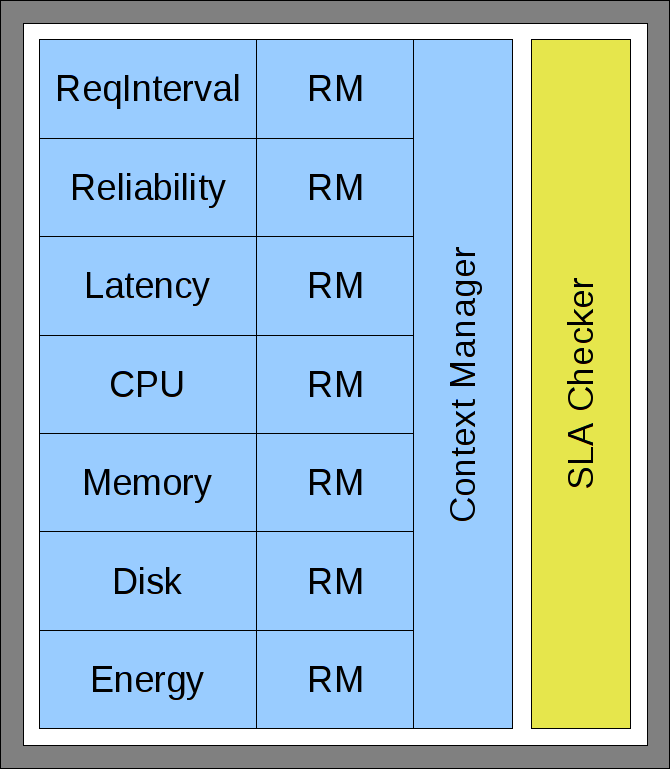
\includegraphics[scale=0.5]{etc/nodo.png}
\caption{Componenti Nodo}
\label{componentinodo}
\end{center}
\end{figure}
Dalla figura \ref{componentinodo} si può notare come è strutturato un singolo nodo, in particolare si può notare come i componenti da monitorare (cpu, memory, disk, energy, latency, reliability, reqInterval) siano in stretto contatto uno a uno con un \var{Resource Monitor}. I \var{Resource Monitor} immettono informazioni dei componenti monitorati sul dsm. Il \var{Context Manager} si occupa di raccogliere tali dati e raggrupparli in un solo oggetto che viene a sua volta immesso sul dsm. Lo \var{SLA Checker} (o \var{SC}), si trova in genere a contatto con il \var{CM} questo perchè raccoglie principalmente le informazioni sul contesto dei vari nodi. Tutte queste parti elencate saranno chiamate d'ora in poi \var{Agenti}, considerando che ci si trova in ambiente di programmazione ad agenti (ovvero \var{Jade}). Gli agenti delle risorse sono stati realizzati per consentire una simulazione più realistica, ovvero ogni agente risorsa non fa altro che generare un valore di utilizzazione basato su vari parametri (ved. cap \ref{cap:modello}).
\subsection{Composizione Rete}
La rete che si è deciso di creare è formata da tanti di questi nodi, sia richiedente che fornitore. Nello specifico ogni nodo fornitore si occupa di fornire un servizio generico, il quale viene registrato nelle pagine gialle del sistema. Ogni richiedente, invece, può richiedere il servizio ad uno qualsiasi dei fornitori disponibili. Questa operazione è stata resa possibile per fare in modo che la simulazione si attenesse ad un tipico caso reale. Per quanto riguarda lo \var{SLA Checker} si è progettato il sistema considerando che tale agente dovesse \var{migrare} da un nodo all'altro in base alle condizioni del contesto. Un esempio della rete in questione con 3 nodi può essere visto in figura \ref{rete}. Si può notare che lo \var{SC} si trova solo su uno dei nodi della rete in quanto deve poter migrare fra di loro.
\begin{figure}[H]
\begin{center}
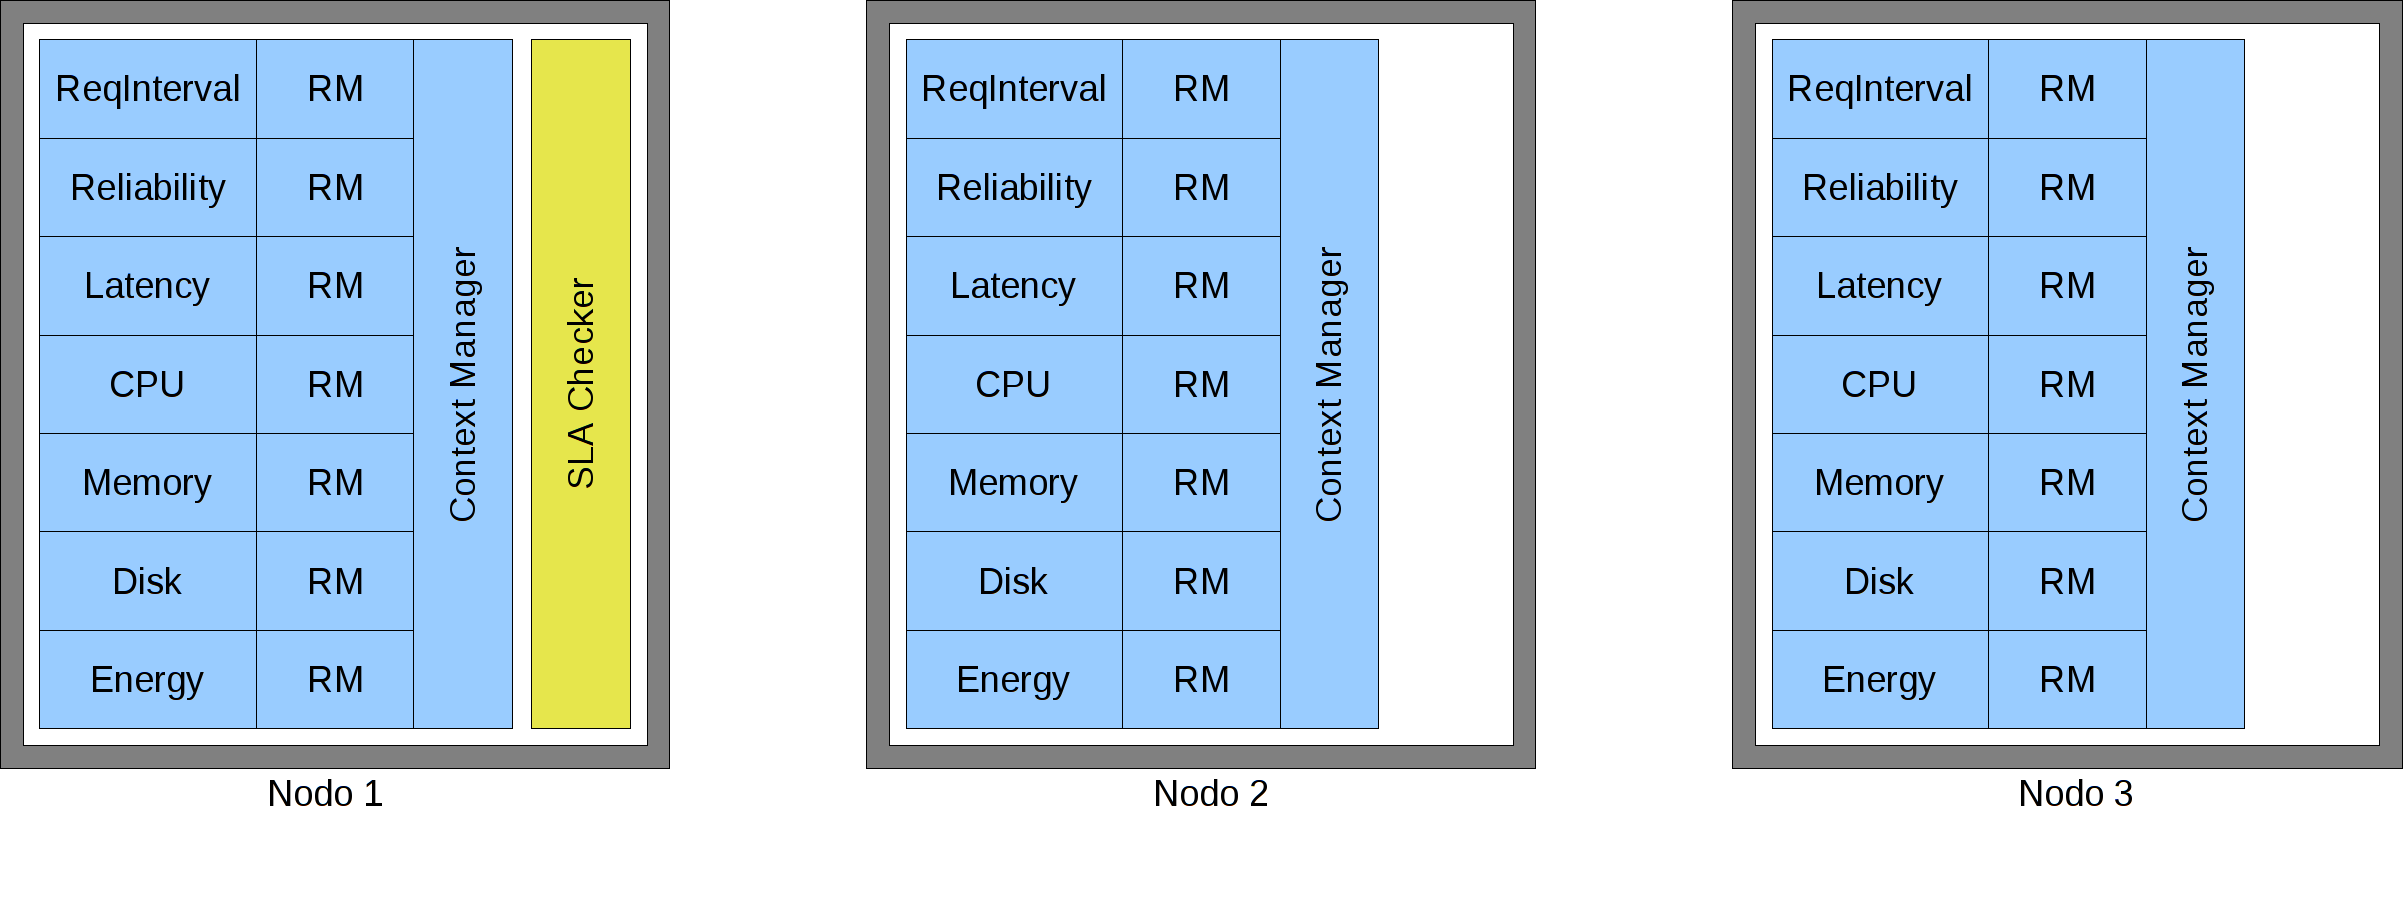
\includegraphics[scale=0.23]{etc/rete.png}
\caption{Esempio di rete con 3 nodi}
\label{rete}
\end{center}
\end{figure}
\section{Funzionamento}
Per spiegare il funzionamento del sistema in questione si è deciso di definire uno scenario d'uso e quindi descrivere il comportamento dei relativi nodi.
\subsection{Scenario d'uso}
Un tipico scenario d'uso potrebbe essere una rete con 3 nodi di cui:
\begin{itemize}
\item 1 nodo fornitore;
\item 2 nodi richiedenti;
\end{itemize}
in particolare ci troviamo in una situazione in cui ognuno dei due nodi richiede un servizio che si attenga al contratto prestabilito con il nodo fornitore. Ogni contratto contiene le seguenti informazioni:
\begin{description}
\item[Publisher:] fornitore del servizio;
\item[Subscriber:] richiedente del servizio;
\item[ReqInterval:] intervallo di tempo tra le richieste del richiedente;
\item[Latency:] tempo impiegato per espletare il servizio;
\item[Reliability:] affidabilità di servizio da parte del fornitore.
\end{description}
Tali informazioni servono per fare in modo che sia il fornitore che il richiedente facciamo il possibile per attenersi ai valori specificati nel contratto.
Su uno dei nodi del sistema è presente lo \var{SLAChecker} che si occupa di controllare la validità di tutti i contratti stipulati; nel caso in cui le condizioni di un contratto vengono violate da uno dei due nodi allora lo \var{SC} informerà immediatamente entrambi i nodi di tale condizione. Tutti i componenti dei nodi sono fortemente dipendenti dalla presenza dello \var{SC}, in quanto comporta un aumento oneroso in termini di calcoli. A causa delle risorse limitate di alcuni nodi (come l'energia) è necessario effettuare un controllo sullo stato attuale dei componenti dei nodi per evitare di sovraccaricarlo, in modo tale che in caso di necessità lo \var{SC} migri su un nodo con condizioni di carico migliori. La selezione del nodo migliore viene fatta utilizzando una specifica politica di selezione (vedi cap. XXX). Un esempio di migrazione può essere visto nelle due figure seguenti, in cui nel primo caso lo SC si trova sul nodo 1, mentre nel secondo caso lo SC è migrato sul nodo 2 a causa di scarsità di risorse sul nodo 1.
\begin{figure}[H]
\begin{center}
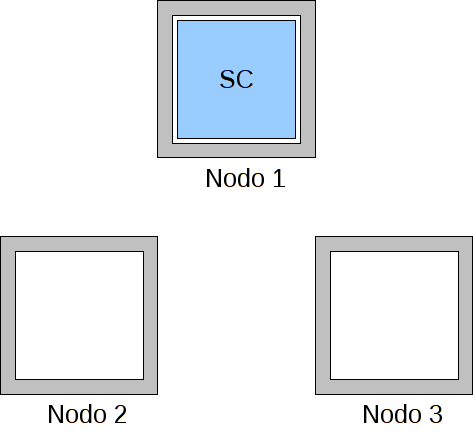
\includegraphics[scale=0.4]{etc/scenario1-1.png}
\caption{Esempio di scenario}
\label{scenario1}
\end{center}
\end{figure}
\begin{figure}[H]
\begin{center}
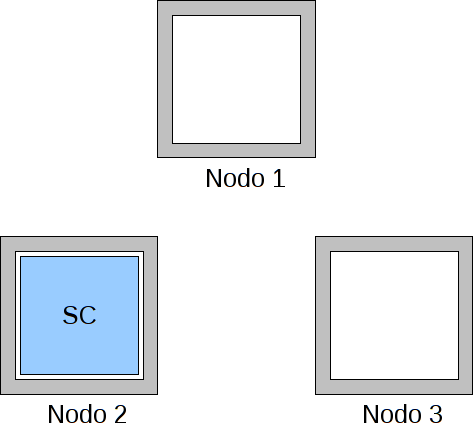
\includegraphics[scale=0.4]{etc/scenario1-2.png}
\caption{Esempio di scenario}
\label{scenario2}
\end{center}
\end{figure}
\subsection{Distribuited Shared Memory}
Per consentire la comunicazione tra i nodi del sistema è stato aggiunto un ulteriore livello nell'architettura in questione, ovvero il \var{dsm}. Tale componente è stato progetto sfruttando i meccanismi di comunicazione di Jade, in particolare lo scambio di messaggi tra server e client dsm avviene tramite messaggi di Jade.
\subsubsection{DsmServer}
E' stato realizzato un agente che si occupa principalmente della ricezione e la computazione delle richieste. Nello specifico quando il server riceve una specifica richiesta effettua la rispettiva operazione sul database dsm.
\subsubsection{DsmData}
Questo componente è necessario per la gestione del dsm e delle tuple, in quanto consente operazioni di \code{IN}, \code{OUT}, \code{UPDATE} e \code{READ}.
\subsubsection{DsmClient}
Quest'ultimo componente è fondamentale per ogni agente che deve inviare o riceve informazioni dal tuple space, infatti consente l'invio delle richieste direttamente all'agente server che provvederà ad esaurirle.
\subsection{Context Manager}
Il Context Manager, come già anticipato, si occupa di raccogliere tutte le informazioni sulle risorse del proprio su un contenitore chiamato \code{Context}, nello specifico il contenuto è il seguente:
\begin{description}
	\item[cpu:] valore del processore;
	\item[ram:] valore della ram presente nel nodo;
	\item[memory:] valore percentuale dell'occupazione di memoria del nodo;
	\item[energy:] valore di energia residua;
	\item[latency:] latenza di trasmissione attuale del nodo publisher;
	\item[reliability:] valore dell'affidabilità del nodo;
	\item[reqInterval:] frequenza di richieste;
	\item[location:] contiene informazioni su cui risiede CM;
	\item[network:] tipo di rete del nodo;
	\item[bandwidth:] banda di rete del nodo.
\end{description}
Per raccogliere tali informazioni il CM effettua delle operazioni di \code{IN} sul dsm ad intervalli predefiniti. Raccolti i dati immette il contesto sul dsm tramite operazioni di \code{OUT}. Il CM si occupa inoltre si richiede ed accettare contratti SLA in base al tipo di nodo in cui si trova, se il nodo è di tipo \var{publisher} accetta contratti invece se è di tipo \var{subscriber} richiede contratti. Una volta accettatto un contratto viene rinviato sul dsm tramite \code{OUT} per essere passato allo SC.
\subsection{SLA Checker}
E' il componente su cui si basa tutto il funzionamento del sistema realizzato, in quanto è l'agente che si occupa di controllare la validità dei contratti e migrare quando necessario. Per effettuare tali operazioni è necessario essere a conoscenza del contesto dei vari nodi e dei contratti SLA stipulati. Lo SC richiede continuamente i contesti dei vari nodi dal dsm, inoltre memorizza tutti i contratti che sono stati stipulati per essere a conoscenza delle relazioni tra i nodi. La conoscenza di tutte le informazioni descritte è necessaria all'algoritmo di \var{checking}, in quanto ha bisogno di tante informazioni per scoprire il miglior nodo su cui migrare (ved. \ref{cap:modello}).
<\chapter{Dsm}
In questo capitolo verrà riportato dettagliatamente il funzionamento e la strutturazione del componente dsm necessario alla comunicazione tra agenti, nello specifico verra spiegato come è stato realizzato il tuple space e tutti i meccanismi ad esso correlati.
Per il progetto in questione sono stati realizzati i comandi prettamente necessari, che sono: IN, OUT, UPDATE e READ \cite{linda}.
\section{DsmData}
Per la gestione dei dati è stato realizzato una sorta di database volatile tramite lo sfruttamento di \var{Hashtable} e \var{Queue}. In particolare si realizzata una struttura del genere:
\begin{figure}[H]
\begin{center}
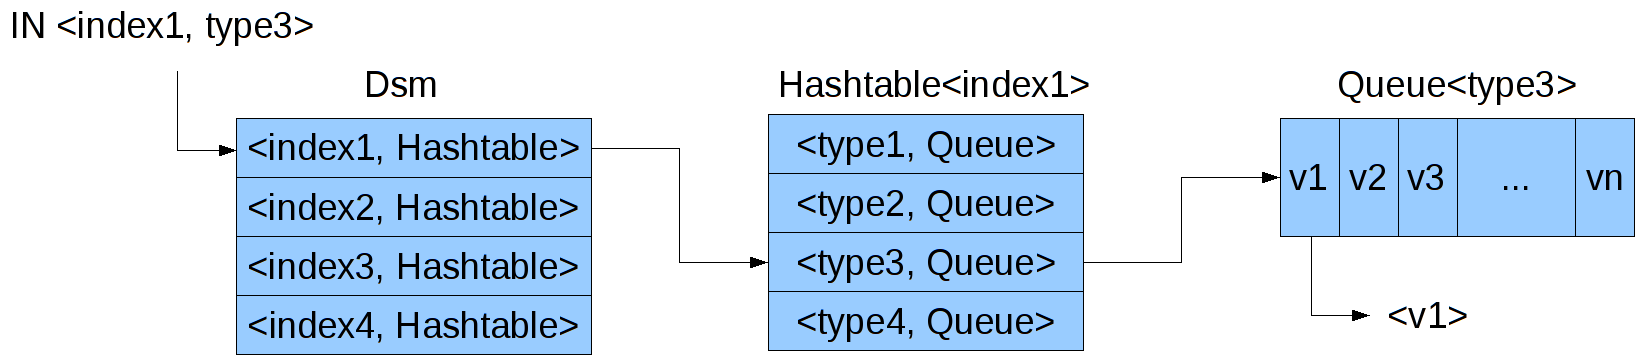
\includegraphics[scale=0.3]{etc/dsm.png}
\caption{Esempio di IN nel Dsm}
\label{dsm1}
\end{center}
\end{figure}
Dalla figura è riportato un esempio delle operazioni eseguite sul database nel momento in cui si effettua una richiesta \code{IN <index1, type3>}, ovvero si richiede un valore di tipo 3 che si trova nell'indice 1. Le operazioni eseguite sono elencate di seguito:
\begin{enumerate}
	\item Quando perviene la richiesta al db si cerca immediatamente la presenza di una chiave \code{index1} nell'hashtable di primo livello;
	\item se la chiave è presente si prende l'hashtable associata e si procede con il controllo delle presenza della chiave \code{type3} all'interno dell'hashtable di secondo livello;
	\item se la chiave è presente si prende la coda che gli è associata e si estrae il valore che si trova in testa.
\end{enumerate}
Operazioni analoghe vengono effettuate per gli altri tipi di operazioni; in particolare le operazioni implementate hanno il seguente comportamento:
\begin{description}
	\item[OUT:] equivale alla tupla \code{OUT <index1, type3, v1>} e consiste nell'inserire un valore sul tuple space.
	\item[IN:] è rappresentata dalla tupla \code{IN <index1, type3>} ed il suo scopo è reperire il valore in testa alla coda e quindi eliminarlo dal tuple space.
	\item[READ:] tupla uguale a IN, ma ha l'unica differenza di non eliminare il valore dopo averlo reperito.
	\item[UPDATE:] tupla come OUT con la differenza che se il valore esiste lo sostituisce.
\end{description}
\section{DsmClient}
Questo componente consente la comunicazione con il server dsm sfruttando lo scambio di messaggi che mette a disposizione Jade con il suo \var{framework}. Il modulo in questione consente due meccanismi principali che sono: l'invio di messaggi bloccanti e l'invio di messaggi non bloccanti. Per quanto riguarda i messaggi bloccanti (IN e READ) si ha:
\begin{enumerate}
	\item Il Client invia la richiesta al server ed attende la risposta;
	\item Il Server riceve la richiesta, la esaurisce ed invia la risposta;
	\item Il Client riceve la richiesta e la ritorna all'agente chiamante.
\end{enumerate}
I messaggi non bloccanti di tipo OUT e UPDATE, invece, vengono inviati nel seguente modo:
\begin{enumerate}
	\item Il Client invia la richiesta al server e ritorna all'agente chiamante;
	\item Il Server riceve la richiesta e la esaurisce;
\end{enumerate}
\section{DsmServer}
Tale componente può essere inteso come un \var{proxy} in quanto non fa altro che tradurre le richieste del client a operazioni sul \code{DsmData} e quindi ritornare una risposta (in caso di messaggi bloccanti). Una caratteristica importante di questo agente è che può migrare tra i vari nodi in base alla disponibilità delle risorse dei nodi, nello specifico non fa altro che seguire lo \var{SC}, ovvero quando lo SC migra su un altro nodo il DsmServer lo segue (rif SC).
\chapter{Modello Matematico}\label{cap:modello}
Il modello matematico riguarda tutta la parte generativa dei valori delle risorse e dell'indice di occupazione dei nodi. Molte delle relazioni che sono state utilizzate sono state ricavate empiricamente grazie ad un operazione di \var{tuning} che ci ha consentito di raggiungere una situazione il più reale possibile.
\section{Valori risorse}
Le risorse del sistema realizzato possono essere suddivise in due gruppi: dipendenti dalla presenza dello SC (e Dsm) e indipendenti dalla loro presenza. Quanto detto è stato fatto per rappresentare più realmente un caso normale. Si consideri il seguente esempio, ovvero un nodo mobile con connessione \var{wireless} e un nodo fisso con connessione \var{wired}. Il nodo mobile viene collegato e scollegato dalla rete elettrica quando necessario. Sul nodo mobile sono in esecuzione delle normali operazioni di richiesta di informazioni verso il nodo fisso. Sul nodo fisso è in esecuzione il server che risponde alle risposte di vari nodi mobili. Lo SC è al momento sul nodo fisso, questo implica un carico computazione molto elevato per tale nodo, quindi se necessario tale agente SC migrerà sul nodo mobile che al momento ha molte risorse disponibili. Per consentire questo meccanismo di migrazione è stato necessario realizzare delle formule di generazione adattabili al loro stato attuale (presenza o non presenza dello SC oppure collegato o scollegato dalla rete elettrica). Tutti i valori generati rappresentano delle percentuali. Di seguito vengono riportate tutte le formule usate per la generazione.
\subsection{Cpu}
La risorsa \var{cpu} dipende fortemente dalla presenza dello SC, infatti si è deciso di applicare la seguenti relazioni, la prima nel caso ``senza SC''
\begin{equation}
cpu = (\alpha \cdot 100) mod 60
\end{equation}
in cui $\alpha$ rappresenta un valore casuale da 0 a 1. Il modulo 60 è stato usato per limitare il valore a 60. Nel caso ``con SC'' invece è stata usata la seguente relazione:
\begin{equation}
cpu = ((\alpha \cdot 100) mod 60) + 40
\end{equation}
in cui si aggiunge il valore 40 che rappresenta il carico supplementare dovuto alla presenza dello SC.
\subsection{Ram}
La risorsa viene generata come per la cpu.
\begin{equation}
ram = (\alpha \cdot 100) mod 60
\end{equation}
Nel caso ``con SC'' invece è stata usata la seguente relazione:
\begin{equation}
ram = ((\alpha \cdot 100) mod 60) + 40
\end{equation}
\subsection{Memory}
La memoria ha un comportamento leggermente più complesso, infatti è stato realizzato un meccanismo di riempimento e svuotamento della memoria dipendente dalla presenza dello SC. All'avvio del nodo viene generato un valore iniziale tramite la seguente formula:
\begin{equation}\label{eq:memory}
memory = (\alpha \cdot 100) mod 60
\end{equation}
Ad ogni \var{tick} si modifica il valore nel seguente modo:
\begin{equation}
memory = memory + 0.2 \cdot ((\alpha \cdot 100) mod 10)
\end{equation}
Quest'ultima relazione consiste nell'aggiungere al valore precedente il $20\%$ di un valore modulo 10, grazie a ciò si ottiene un incremento molto lieve dell'utilizzazione della memoria.
Nel caso ``senza SC'' invece si ha
\begin{equation}
memory = memory - 0.2 \cdot ( ( \alpha \cdot 100 ) mod 10 )
\end{equation}
a differenza del caso precedente si sottrae il nuovo valore da quello vecchio, questo sta ad indicare una diminuzione dell'utilizzazione. Inoltre nel caso in cui la memoria raggiunge valori minori di 0 o maggiori 100 si rigenera il valore della memoria con la formula usata inizialmente (ved. \ref{eq:memory}).
\subsection{Energy}
Nel caso del componente riguardante l'energia sono state applicate delle formule più adattative, in quanto il suo valore dipende dal collegamento o scollegamento alla rete elettrica e dalla presenza o non presenza dello SC. Inoltre dipende dal tipo di connessione, ovverro se è wireless o wired. All'avvio viene generato il valore tramite la seguente formula.
\begin{equation}\label{eq:energy}
memory = (\alpha \cdot 100) mod 60
\end{equation}
Ad ogni tick dell'agente si può avere una delle seguenti formule in base alle condizioni. In caso di connessione wired si ha:
\begin{equation}
energy = 100
\end{equation}
considerando che il wired è stato assunto come nodo fisso collegato alla rete elettrica. In caso di connessione wireless si deve distinguere dal caso in cui è connesso alla rete elettrica (\code{powerOn}) e il caso in cui non lo è (\code{!powerOn}). Per rendere reale i valori generati si è realizzato un meccanismo per gestire la connessione e sconnessione dalla rete elettrica, ovvero:
\begin{gather}
\text{se }energy \leq 10\text{ then }powerOn = true \\
\text{se }energy \geq 99\text{ then }powerOn = false
\end{gather}
Con la rete elettrica collegata si ha:
\begin{gather}
energy = energy + 0.8 \text{ se SC non presente},\\
energy = energy + 0.6 \text{ se SC presente}
\end{gather}
in caso di rete elettrica scollegata si ha:
\begin{gather}
energy = energy - 0.2 \text{ se SC non presente},\\
energy = energy - 1 \text{ se SC presente}
\end{gather}
\subsection{Latency}
Nel caso della latenza è stato usato un meccanismo dipendente solo dalla presenza dello SC e dal tipo di connessione. In particolare se nel nodo è presente lo SC oppure ha una connessione wireless si ha:
\begin{equation}
latency = ((\alpha_{1} \cdot 100)mod60) + \left( \left(\frac{\alpha_{2} \cdot 100}{\frac{\beta}{50}}\right)mod40\right)
\end{equation}
come si può notare vengono generati due numeri, uno modulo 60 ed uno modulo 40 in modo da avere un numero massimo di 100. Inoltre è presente un valore $\beta$ che rappresenta la banda del nodo.
\subsection{Reliability}
Il valore della affidabilità del canale viene generato nello stesso modo della latenza, infatti si ha:
\begin{equation}
reliability = ((\alpha_{1} \cdot 100)mod60) + \left( \left(\frac{\alpha_{2} \cdot 100}{\frac{\beta}{50}}\right)mod40\right)
\end{equation}
\subsection{ReqInterval}
In quest'ultima risorsa la generazione avviene molto semplicemente generando un numero casuale da 0 a 100.
\begin{equation}
reqInterval = \alpha \cdot 100
\end{equation}
\section{SLA Checker}
Lo SC essendo il componente centrale di tutto il sistema ha richiesto un lavoro molto accurato per la realizzazione di un buon algoritmo e di un indice di valutazione efficiente. Per algoritmo si intendono le operazioni che vengono svolte dallo SC ciclicamente (ad ogni tick dell'agente), ovvero il controllo sulla validità dei contratti e il controllo della necessità di migrazione. Per indice di valutazione si intende il valore che viene generato per ogni nodo dai valori del suo contesto, tale indice viene utilizzato dallo SC per trovare il nodo su cui eventualmente migrare.
\subsection{Algoritmo controllo}
L'algoritmo realizzato consente il controllo della violazione dei contratti e il controllo della necessità di migrazione. In particolare tali operazioni possono essere effettuate grazie alla conoscenza di tutte le informazioni sui nodi del sistema, ovvero il contesto e i contratti. L'algoritmo è suddiviso in due parti, la prima si occupa del controllo della validità dei contratti.
\subsubsection{SLA Contract checking}
\begin{enumerate}
	\item si prende un contratto SLA dalla lista dei contratti;
	\item si recuperano i dati del contesto dei due partecipanti al contratto (Publisher, Subscriber);
	\item si controlla la validità del contratto tramite la relazione seguente:
		$$
			latency_{pub} > latency_{sla}
		$$
			\centering{OR}
		$$
			reliability_{pub} > reliability_{sla}
		$$
			\centering{OR}
		$$
			reqInt_{sub} > reqInt_{sla}
		$$
	\item se tale relazione risulta valida allora il contratto è stato violato.
\end{enumerate}
Dalla relazione riportata si può notare la presenza dei valori di \code{latency}, \code{reliability} e \code{reqInt} che hanno come pedice \code{pub}, \code{sub} e \code{sla} che indicano rispettivamente il Publisher, il Subscriber e il contratto SLA. La relazione riportata non fa altro che controllare se il publisher viola il contratto non garantendo la latenza e l'affidabilità precedente, oppure se il Subscriber viola il contratto effettuando più richieste di quante stabilite dal contratto SLA.
\subsubsection{SC Migration checker}
La seconda parte di cui si occupa lo SC è la verifica della necessità di migrazione su altri nodi. In particolare tale operazione consiste nel valutare l'indice del contesto di ogni nodo, controllando se il valore supera una certa soglia prefissata, nel qual caso sarebbe necessario migrare su un nuovo nodo. Il calcolo dell'indice di utilizzazione viene effettuato con la seguente formula:
\begin{equation}\label{eq:index}
index = cpu \cdot 0.23 + ram \cdot 0.23 + memory \cdot 0.23 + (100-energy) \cdot 0.3
\end{equation}
Il valore $index$ calcolato rappresenta una percentuale che va da 0 a 100 che indica l'utilizzazione del nodo valutato. L'indice è il fulcro dell'algoritmo di \var{Migration checking}, in quanto la migrazione si basa proprio sul confronto di tale valore. Verranno ora riportati i passi dell'algoritmo:
\begin{enumerate}
	\item Innanzitutto si recupera il nodo migliore su cui migrare tramite la funzione \code{getBestNode()};
	\item si seleziona il contesto attuale del nodo in cui si trova lo SC;
	\item si verifica che l'indice del contesto attuale sia maggiore dell'indice di migrazione;
	\item se la condizione è verificata si effettua la migrazione sul nodo risultato migliore;
	\item si notifica, tramite dsm, l'avvenimento della migrazione a tutti nodi presenti;
	\item se la condizione non si verifica non viene effettuata la migrazione.
\end{enumerate}
\subsubsection{Best Node}
La funzione \code{getBestNode()} riportata nell'algoritmo precedente viene descritta dettagliatamente di seguito:
\begin{lstlisting}[frame=trBL]
AID next, iter;
Enumeration<AID> keys = sc.getContextTable().keys();
Context context;
float cpu, ram, memory, energy;
float total=500, iter=0;

while(keys.hasMoreElements()) {
  next = keys.nextElement();
  context = sc.getContextTable().get(next);
  if(context!=null) {
    cpu = context.getCpu();
    ram = context.getRam();
    memory = context.getMemory();
    energy = context.getEnergy();
    iter = cpu + ram + memory + (1-energy);
    if(cpu < Context.CPU_LIMIT && ram < Context.RAM_LIMIT && memory < Context.MEMORY_LIMIT && energy > Context.ENERGY_LIMIT && iter < total) {
      best = next;
      total = iter;
    }
  }
}
\end{lstlisting}
Lo scopo dell'algoritmo riportato è di recuperare il contesto che ha i valori ``migliori'', ovvero che si attiene alla seguente relazione:
$$
cpu < cpu_{limit} \;AND\; ram < ram_{limit}\; AND
$$
$$
memory < memory_{limit} \;AND\; energy > energy_{limit}\; AND\; \theta < min
$$
in cui i valori con pedice $limit$ indicano il massimo numero per cui si accetta il valore come ``migliore''. $\theta$ invece rappresenta il minimo attuale, calcolato tramite \ref{eq:iter}
\begin{equation}\label{eq:iter}
\theta = cpu + ram + memory + (1-energy)
\end{equation}
in ogni ciclo viene calcolato tale valore e se risulta essere minore del minimo attuale si sostituisce $min$ con tale valore.
\chapter{Implementazione}
Questo capitolo consente di avere una panoramica sull'implementazione, in particolare viene riportato lo schema \var{UML} delle dipendenze tra i package per avere un'idea di come è strutturato il sistema.
\begin{figure}[H]
\begin{center}
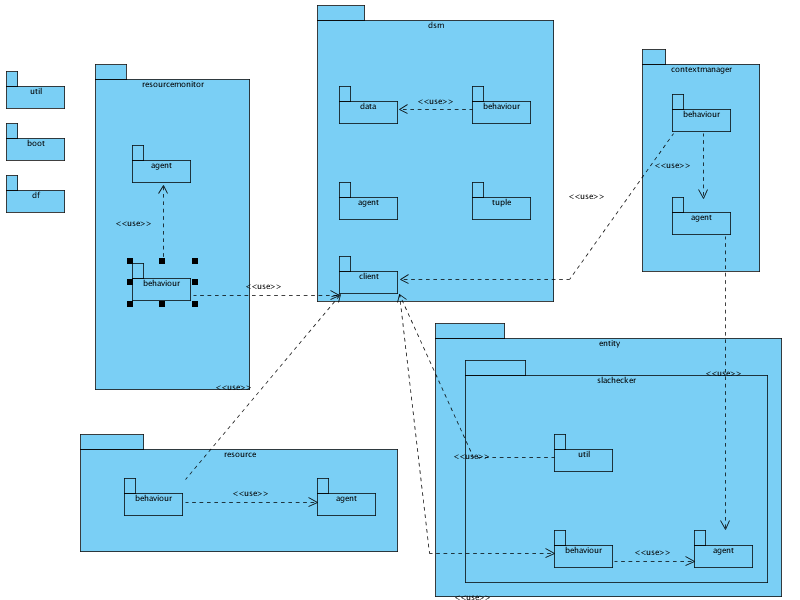
\includegraphics[scale=0.4]{etc/diagramm1.png}
\caption{Relazioni tra Package}
\label{fig:package}
\end{center}
\end{figure}
\chapter{Simulazione}
Per valutare le prestazioni del sistema realizzato si sono effettuate numerose simulazioni. Tutti i test condotti sono stati basati su una specifica configurazione di nodi, in particolare 1 nodo Publisher e 2 Subscriber. I due nodi consumer richiedono la stipulazione di un contratto al producer, il quale espleta tutte le richieste. Si riporta ora un esempio di esecuzione con relativa descrizione ed analisi dei dati.
\section{Esecuzione}
In principio si avvia il nodo Producer il quale andrà in attesa di richieste dei consumatori. In seguito si avviano i due Consumer (o Subscriber) i quali richiedono ed ottengono un contratto con il Subscriber. Stabiliti i contratti inizia la vera fase di simulazione in cui ogni nodo genera valori casuali per le proprie risorse e lo SC raccoglie tali dati per valutare gli SLA e la necessità di migrazione. Per eseguire il sistema bisogna utilizzare i seguenti comandi;
\begin{verbatim}
ant runGui
\end{verbatim}
per avviare il \code{MainContainer}
\begin{verbatim}
ant -f build2.xml AgentLauncher
\end{verbatim}
che avvia i tre nodi in tre container differenti.
\subsection{Scenario}
I tre nodi dello scenario d'esecuzione hanno le seguenti caratteristiche:
\begin{enumerate}
	\item Publisher con connessione WIRED e 512Kb di banda;
	\item subscriber con connessione WIRELESS e 256Kb di banda;
	\item subscriber con connessione WIRELESS e 256Kb di banda.
\end{enumerate}
\subsection{Generazione contratti SLA}
Il contratto SLA, ovvero i livelli di latency, reliability e reqInterval vengono generati casualmente dal publisher nel momento in cui raccolgono una richiesta di contratto. Tale operazione può essere vista nel log di esecuzione del programma simulativo.
\begin{enumerate}
\item Il Subscriber richiede un contratto con un qualsiasi publisher disponibile;
\item Il publisher legge la richiesta dal dsm;
\begin{center}
\begin{verbatim}
SLAContract-request received from cm2
\end{verbatim}
\end{center}
\item il publisher genera i parametri del contratto casualmente e lo immette sul dsm;
\item lo SC rileva la presenza del contratto e lo aggiunge alla sua lista.
\begin{center}
\begin{verbatim}
Added Contract
\end{verbatim}
\end{center}
\end{enumerate}
\subsection{Migrazione}
Inizialmente lo SC risiede sul primo nodo, ovvero il publisher (ved. \ref{fig:primo}).
\begin{figure}[H]
\begin{center}
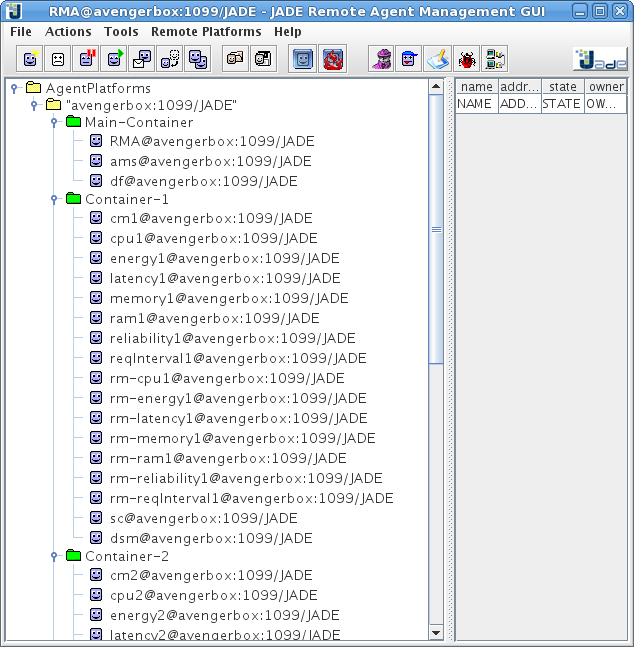
\includegraphics[scale=0.5]{etc/primo.png}
\caption{Migrazione non avvenuta}
\label{fig:primo}
\end{center}
\end{figure}
In questa figura si può notare la presenza del dsm e dello SC sul primo nodo, in quanto la simulazione è stata appena avviata. Dal log si può rilevare che lo SC ha già iniziato a controllare la necessità di migrazione e che al momento si trova sul Container-1 ovvero il nodo 1. Il valore index del nodo attuale non ha ancora superato il valore di soglia (52), di conseguenza lo SC rimane sul nodo attuale.
\begin{lstlisting}
Sono su Container-1
Context[cm3]--> cpu: 40.092556, ram: 16.937687, memory: 34.849556, energy: 81.61731, index: 26.647161
Context[cm1]--> cpu: 57.77024, ram: 51.60415, memory: 45.732647, energy: 100.0, index: 35.674618
Context[cm2]--> cpu: 4.5756726, ram: 52.93144, memory: 40.222347, energy: 98.34838, index: 22.97326
Associated with: cm1
Actual context--> cpu: 57.77024, ram: 51.60415, memory: 45.732647, energy: 100.0, index: 35.674618
\end{lstlisting}
Nel momento in cui il carico su tale nodo raggiunge valori troppo alti avverrà la migrazione. Infatti poco tempo dopo si ha una situazione del genere:
\begin{lstlisting}
Sono su Container-1
Context[cm3]--> cpu: 10.354793, ram: 26.346369, memory: 2.7747908, energy: 75.6174, index: 16.394249
Context[cm1]--> cpu: 77.09479, ram: 64.88432, memory: 87.20903, energy: 100.0, index: 52.713272
Context[cm2]--> cpu: 5.725228, ram: 59.014675, memory: 7.089407, energy: 92.148476, index: 18.876198
Associated with: cm1
Actual context--> cpu: 77.09479, ram: 64.88432, memory: 87.20903, energy: 100.0, index: <52.713272>
Migration to cm3
Moving DSM to 3

Sono su Container-3
Context[cm1]--> cpu: 7.0192904, ram: 18.302485, memory: 86.83973, energy: 100.0, index: 25.797146
Context[cm2]--> cpu: 25.42843, ram: 30.698774, memory: 4.063858, energy: 91.34849, index: 16.4394
Context[cm3]--> cpu: 3.4131508, ram: 16.183126, memory: 7.618082, energy: 74.61742, index: 13.874079
Associated with: cm3
Actual context--> cpu: 3.4131508, ram: 16.183126, memory: 7.618082, energy: 74.61742, index: <13.874079>
\end{lstlisting}
l'indice sul nodo attuale ha raggiunto un valore di 57.71 a causa di un elevato uso delle risorse disponibili, in particolare della della memoria. Dalla figura \ref{fig:secondo} si può notare che il dsm e lo SC si sono spostati sul Container-3. Su quest'ultimo nodo l'indice è adesso di 21.1.
\begin{figure}[H]
\begin{center}
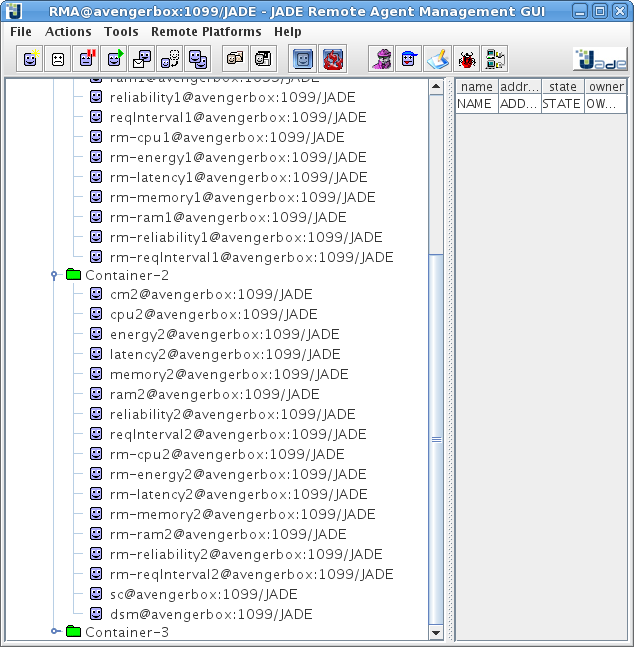
\includegraphics[scale=0.5]{etc/secondo.png}
\caption{Migrazione su secondo nodo}
\label{fig:secondo}
\end{center}
\end{figure}
Il nodo 3 è di tipo WIRELESS e quindi ha una energia limitata, il che implica un tempo di residenza per l'SC e il dsm molto più ridotto, in quanto l'indice raggiungerà rapidamente valori alti.
\begin{lstlisting}
Sono su Container-3
Context[cm1]--> cpu: 0.81155604, ram: 33.999382, memory: 51.11227, energy: 100.0, index: 19.762337
Context[cm2]--> cpu: 36.432972, ram: 58.424694, memory: 1.620206, energy: 84.948586, index: 26.705338
Context[cm3]--> cpu: 67.67117, ram: 95.22946, memory: 26.253895, energy: 49.21744, index: 58.74031
Associated with: cm3
Actual context--> cpu: 67.67117, ram: 95.22946, memory: 26.253895, energy: 49.21744, index: <58.74031>
Migration to cm1
Moving DSM to 1

Sono su Container-1
Context[cm1]--> cpu: 50.261562, ram: 62.669903, memory: 48.456142, energy: 100.0, index: 37.11915
Context[cm2]--> cpu: 1.1113803, ram: 6.8676476, memory: 18.00424, energy: 83.9486, index: 10.791573
Context[cm3]--> cpu: 83.216156, ram: 71.41142, memory: 32.01974, energy: 44.21744, index: 59.663654
Associated with: cm1
Actual context--> cpu: 50.261562, ram: 62.669903, memory: 48.456142, energy: 100.0, index: <37.11915>
\end{lstlisting}
L'energia del nodo 3 è scesa da 49 a 44 il che ha costretto la migrazione sul nodo meno carico, ovvero l'uno (WIRED). In seguito vi è stata anche una violazione del contratto ed è stata segnalata ad entrambi i nodi partecipanti al contratto, i quali dovranno adattarsi per evitare di ripetere la violazione.
\begin{lstlisting}
Violated with latency 23.106468 > 82.419365, reliability 41.978447 > 99.44324, reqInterval 79.21008 > 76.23332
\end{lstlisting}
Dal log si può notare che è stato il subscriber ad eccedere in rischieste, infatti il reqInterval è inteso come frequenza.
\section{Analisi dati}
In questa sezione verranno esposti e commentati i grafici relativi alla simulazione, in quanto molto più esplicativi dei log riportati sopra. Tutti i grafici riportati avranno come ascisse i secondi che non rappresentato un valore reale ma simulato, infatti servono per dare un senso più reale alla simulazione. 
\subsection{Indice}
L'indice è il valore più importante del test eseguito, in quanto la migrazione si basa su di esso. Come passo fondamentale vengono ora riportati i grafici relativi agli indici.
\begin{figure}[H]
\begin{center}
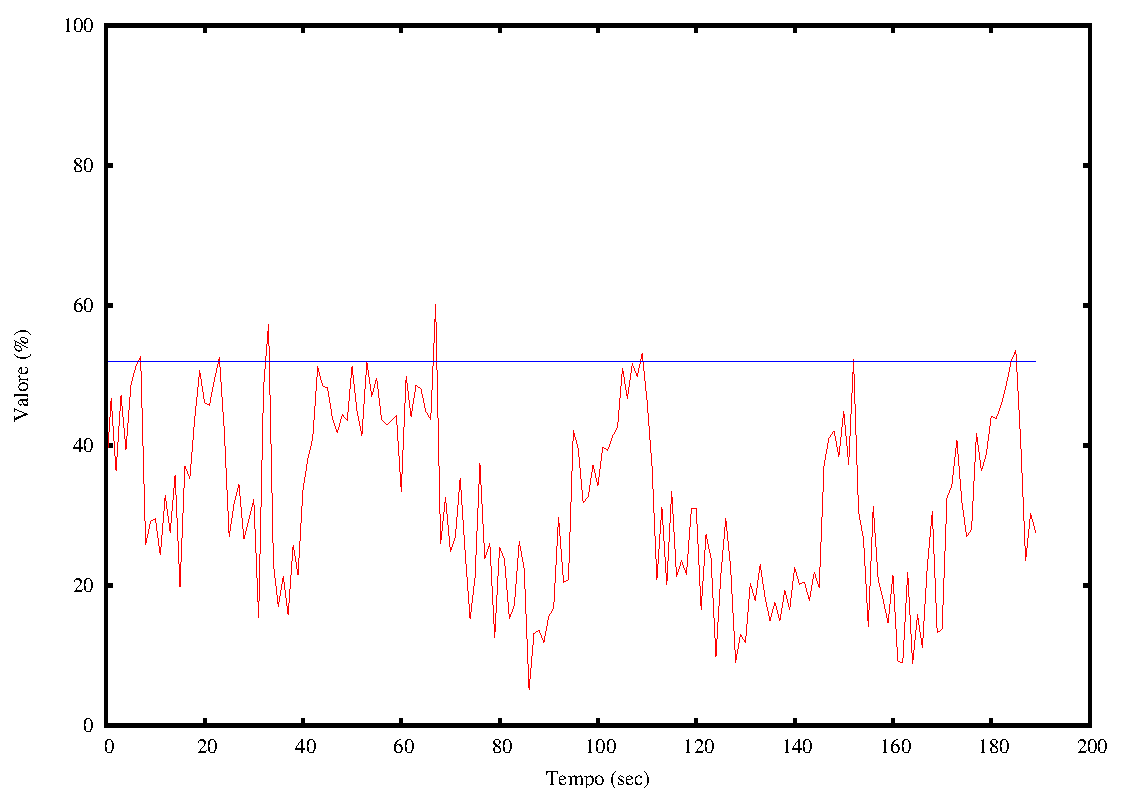
\includegraphics[scale=0.6]{etc/index1.pdf}
\caption{Indice primo nodo}
\label{fig:index1}
\end{center}
\end{figure}
\begin{figure}[H]
\begin{center}
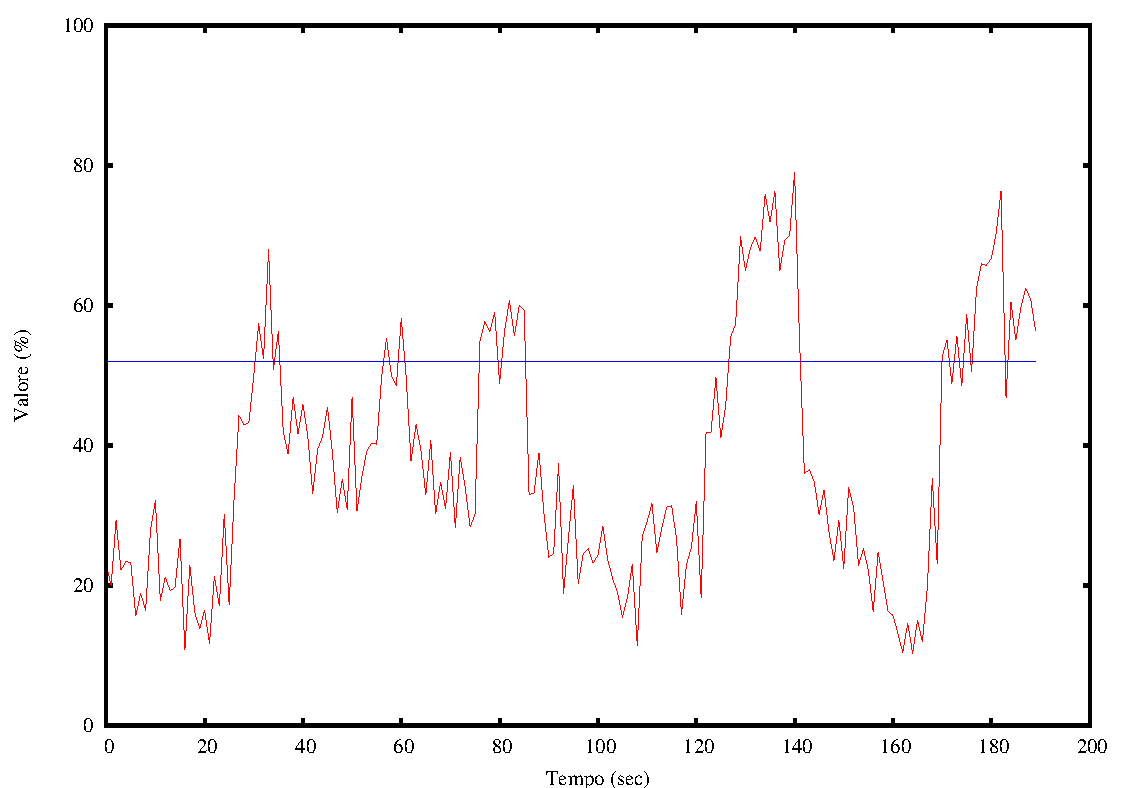
\includegraphics[scale=0.6]{etc/index2.pdf}
\caption{Indice secondo nodo}
\label{fig:index2}
\end{center}
\end{figure}
\begin{figure}[H]
\begin{center}
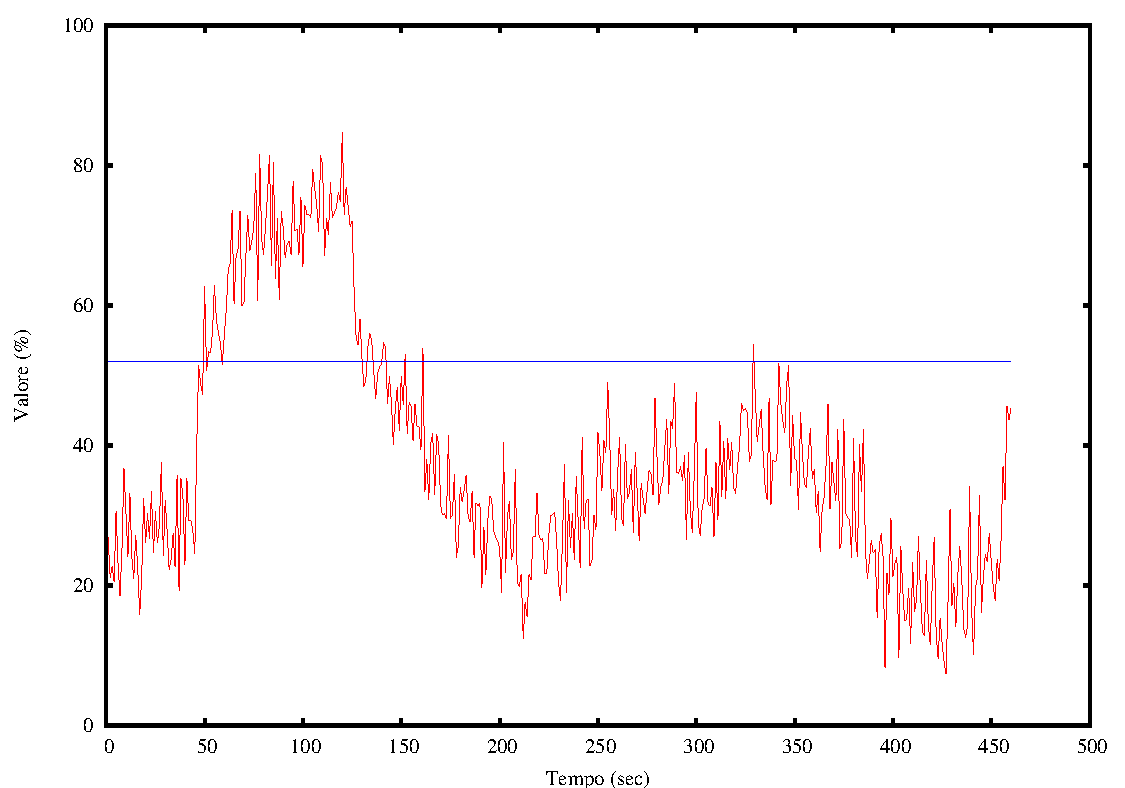
\includegraphics[scale=0.6]{etc/index3.pdf}
\caption{Indice terzo nodo}
\label{fig:index3}
\end{center}
\end{figure}
\begin{figure}[H]
\begin{center}
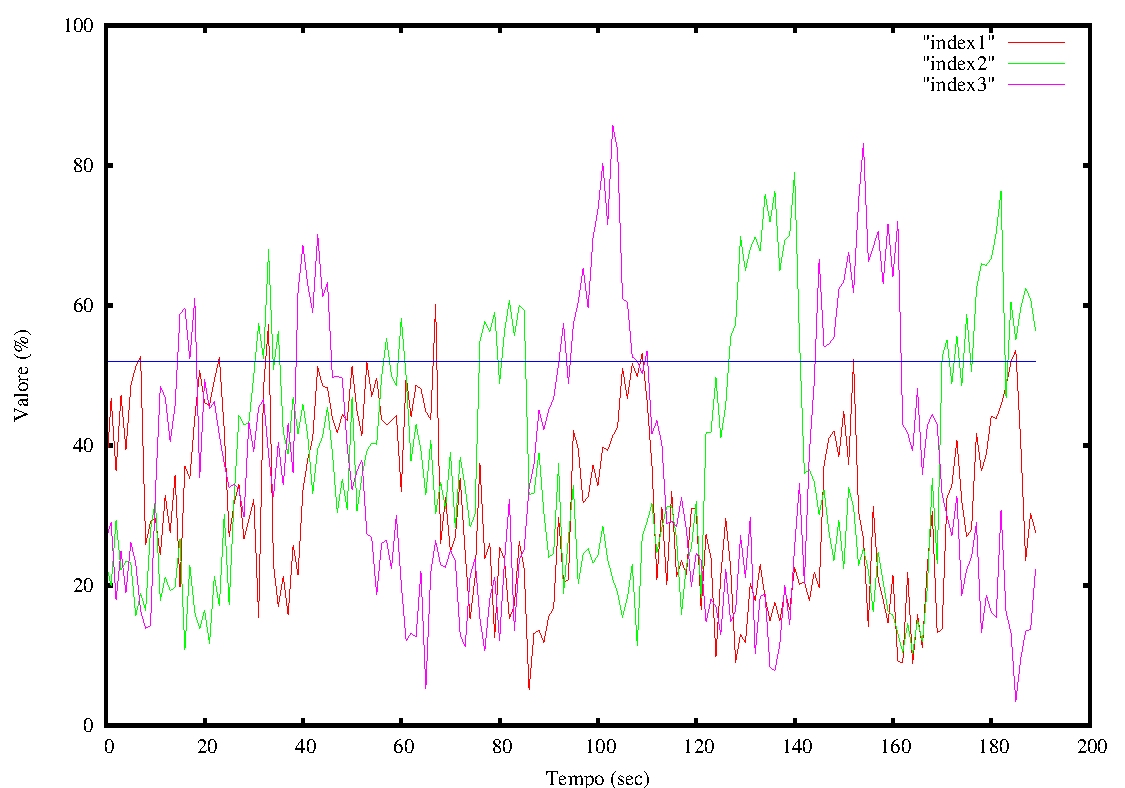
\includegraphics[scale=0.6]{etc/index.pdf}
\caption{Indice tutti i nodi}
\label{fig:index}
\end{center}
\end{figure}
Nelle figure \ref{fig:index1}, \ref{fig:index2}, \ref{fig:index3} e \ref{fig:index} si può notare la presenza di una retta di colore blu, questa rappresenta il limite dell'indice, ovvero 52. Per comprendere meglio i grafici basta sapere che quando i punti superano la retta blu si ha una migrazione dal nodo corrispondente ad un altro. Ad esempio in figura \ref{fig:index1} avviene la prima migrazione al secondo 8 circa.

\subsection{Cpu}
La cpu è molto sensibile alla migrazione, infatti quando lo SC si trova su un nodo si può notare un incremento del 40\% sull'utilizzazione della cpu locale. Tale comportamento può essere facilmente estrapolato dai grafici riportati.
\begin{figure}[H]
\begin{center}
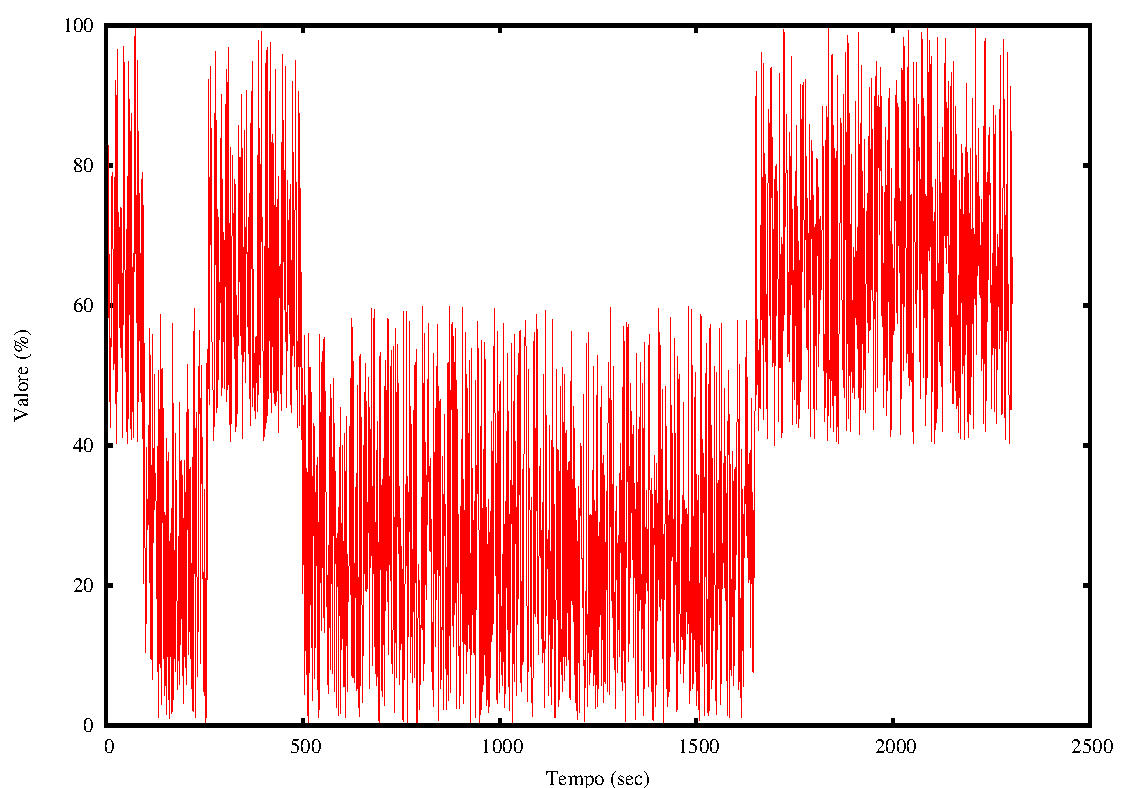
\includegraphics[scale=0.6]{etc/cpu1.pdf}
\caption{Cpu primo nodo}
\label{fig:cpu1}
\end{center}
\end{figure}
\begin{figure}[H]
\begin{center}
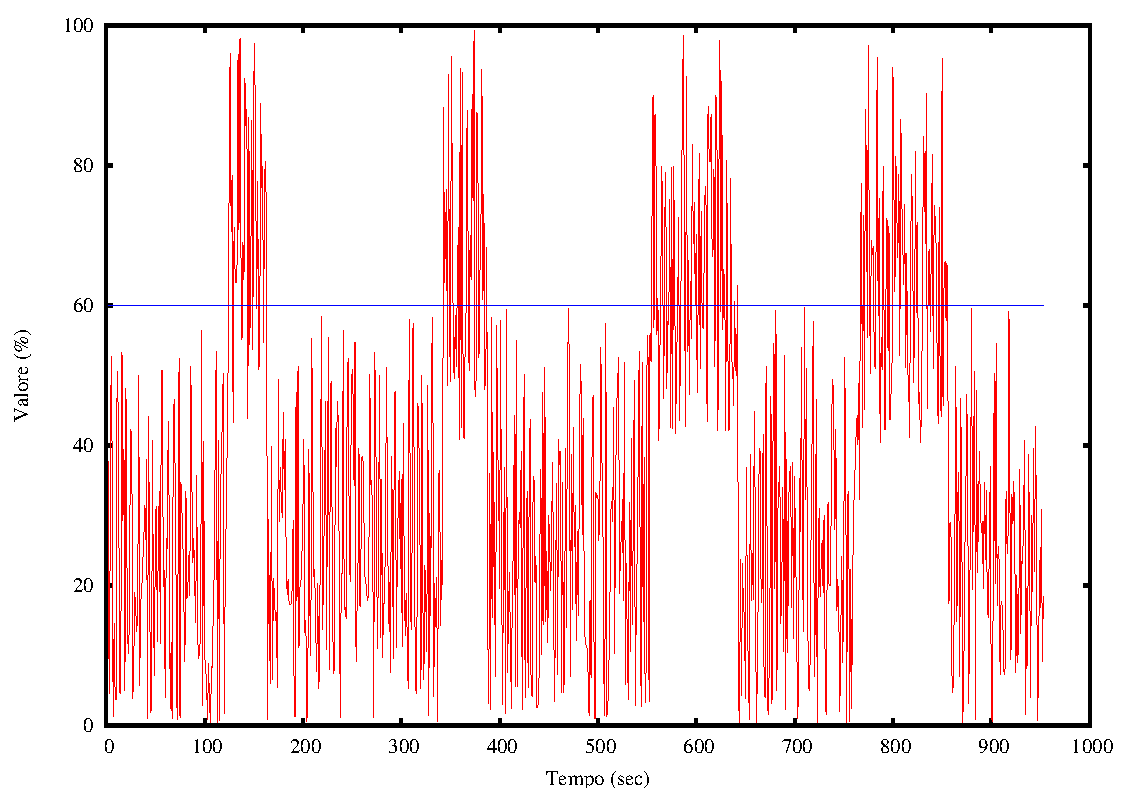
\includegraphics[scale=0.6]{etc/cpu2.pdf}
\caption{Cpu secondo nodo}
\label{fig:cpu2}
\end{center}
\end{figure}
\begin{figure}[H]
\begin{center}
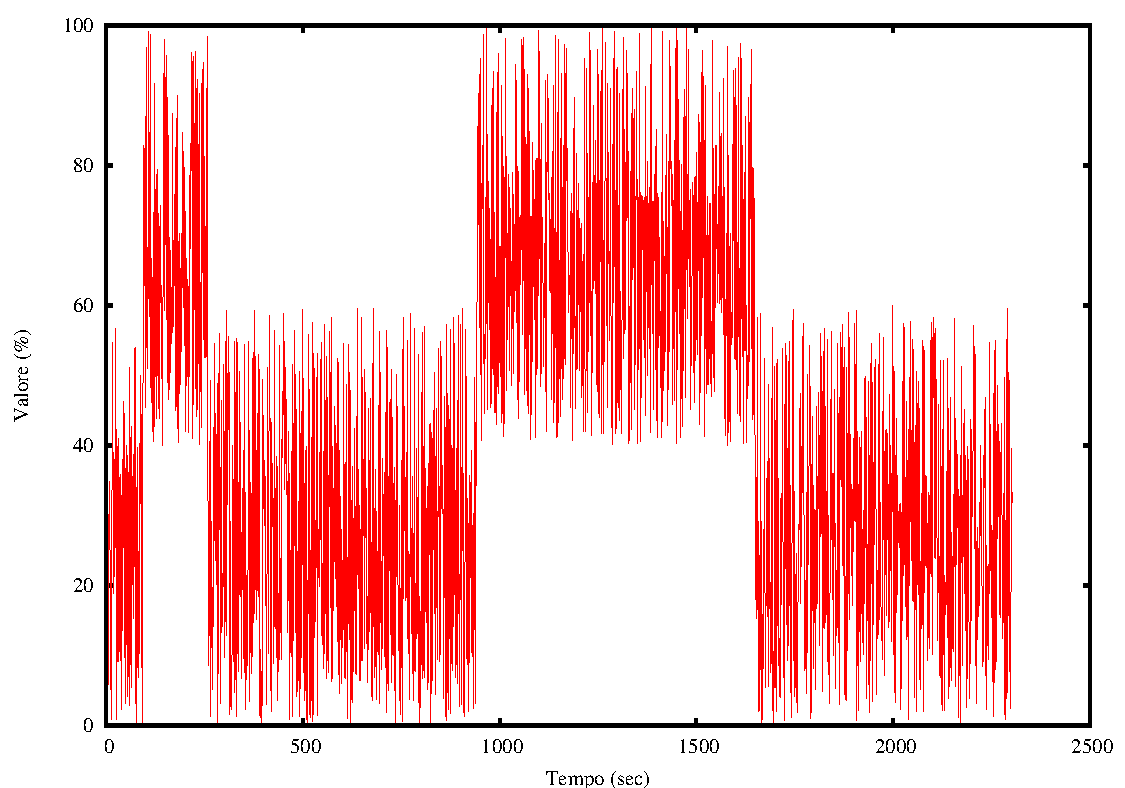
\includegraphics[scale=0.6]{etc/cpu3.pdf}
\caption{Cpu terzo nodo}
\label{fig:cpu3}
\end{center}
\end{figure}
\begin{figure}[H]
\begin{center}
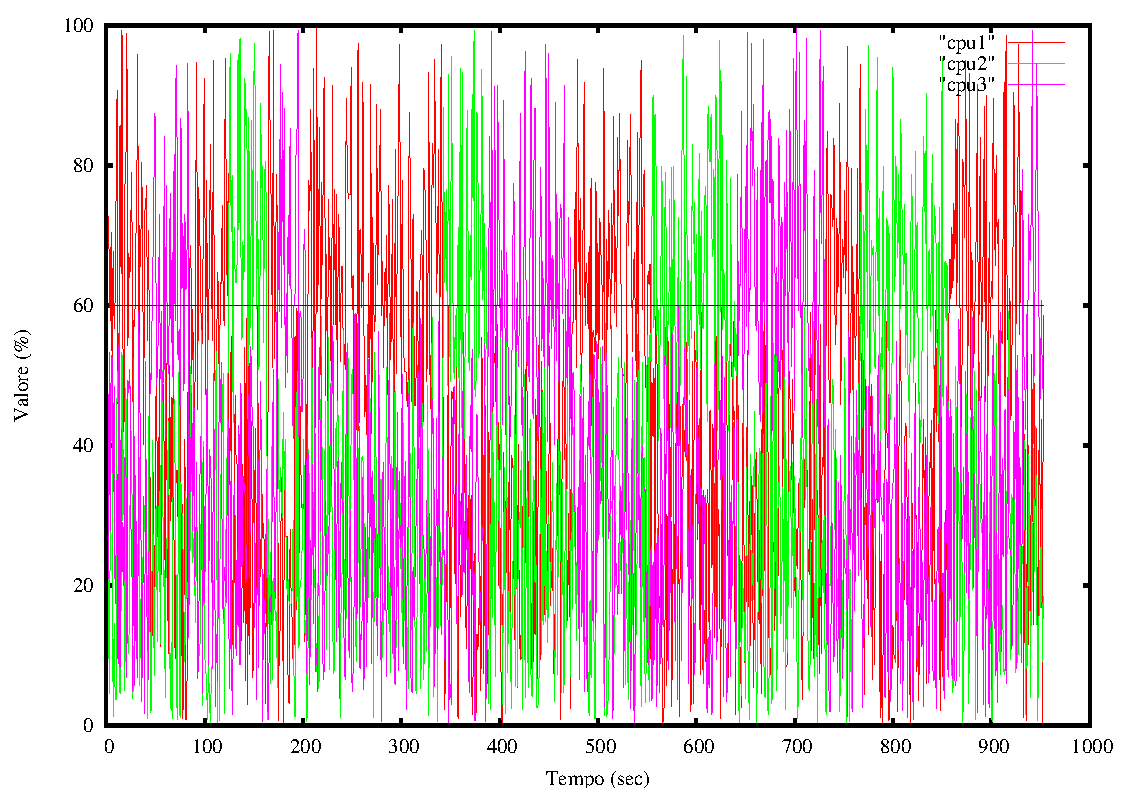
\includegraphics[scale=0.6]{etc/cpu.pdf}
\caption{Cpu tutti i nodi}
\label{fig:cpu}
\end{center}
\end{figure}
In tali grafici è presente una retta sul valore 60\% per distinguere il i nodi che hanno lo SC dagli altri, in particolare quando i valori si trovano oltre 60\% è presente lo SC sul nodo corrispondente. In presenza di una migrazione avviene un brusco cambiamento di carico, infatti si scende sotto il 60\%. Nella figura \ref{fig:cpu} sono graficati i tre nodi, questo crea confusione ma rende più semplicemente l'idea di come migri lo SC da un nodo ad un altro. Nello specifico si può notare che nella parte superiore al 60\% si trova sempre un nodo nel singono istante di tempo, questo è causato dalla presenza di un solo SC che si muove tra i nodi.

\subsection{Ram}
La ram ha una sensibilità come la cpu, infatti i valore vengono generati con le stesse formule. Dai grafici che seguono si possono notare i picchi di carico in corrispondenza delle migrazioni.
\begin{figure}[H]
\begin{center}
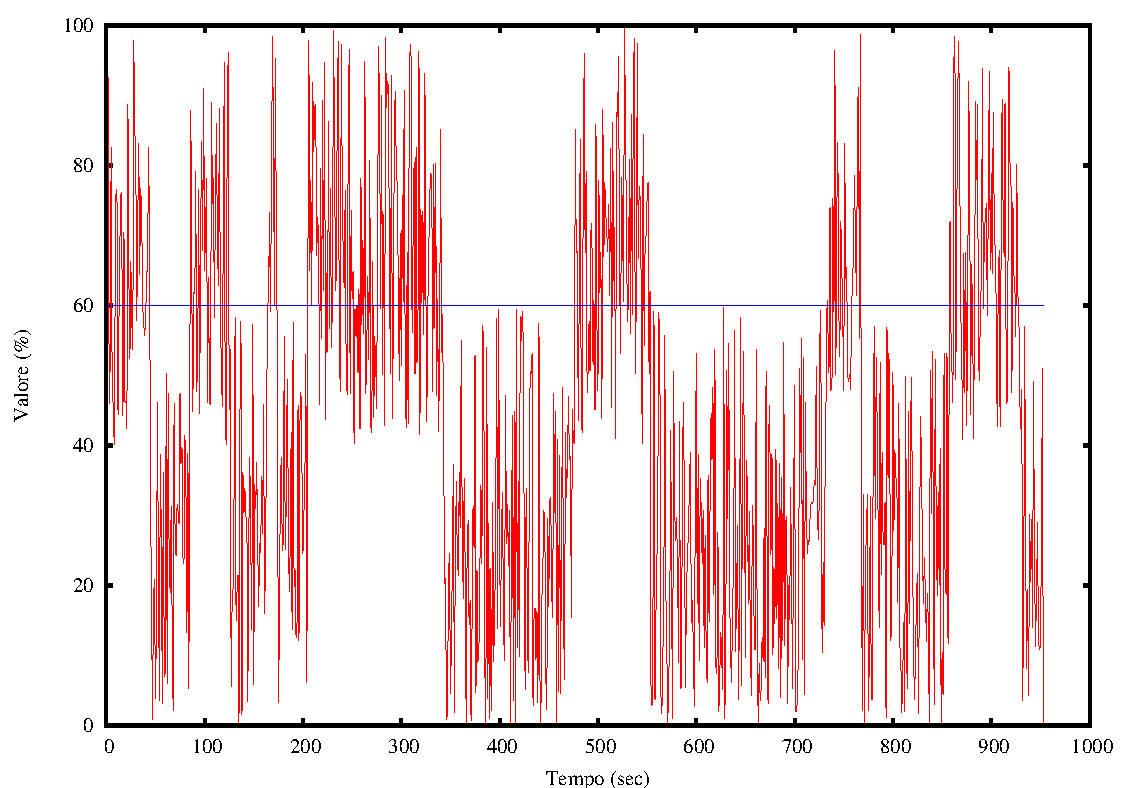
\includegraphics[scale=0.6]{etc/ram1.pdf}
\caption{Ram primo nodo}
\label{fig:ram1}
\end{center}
\end{figure}
\begin{figure}[H]
\begin{center}
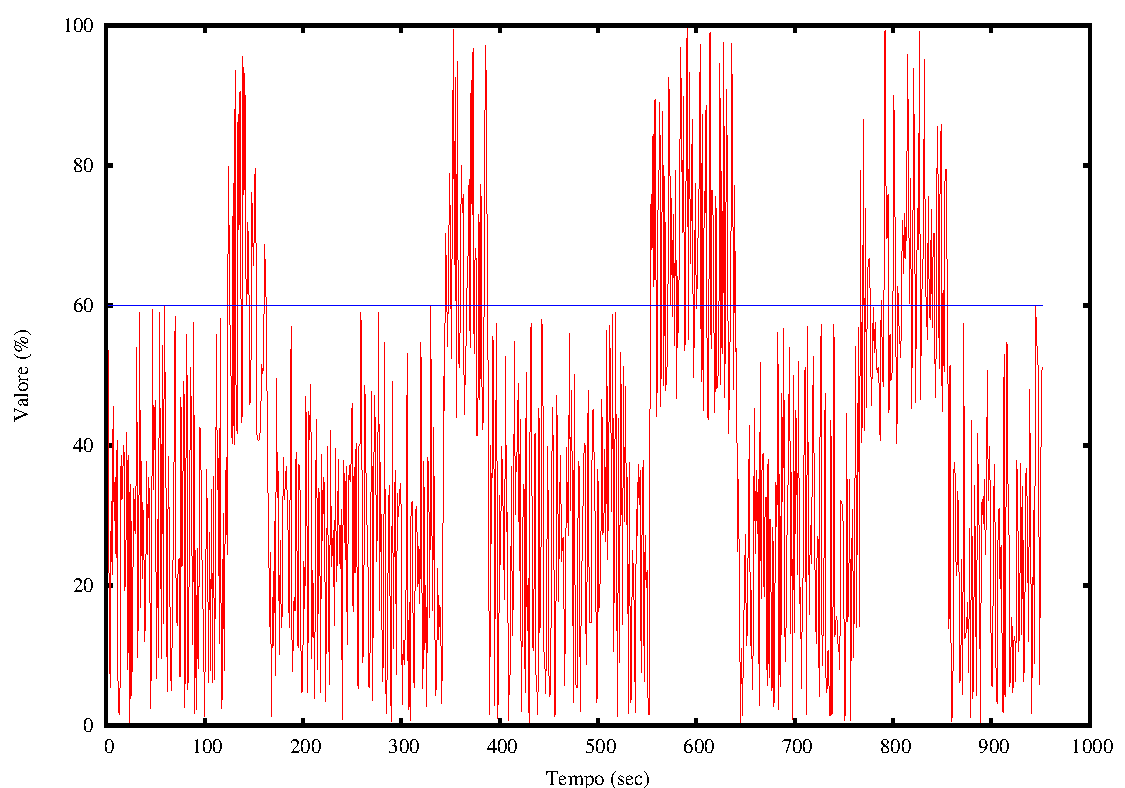
\includegraphics[scale=0.6]{etc/ram2.pdf}
\caption{Ram secondo nodo}
\label{fig:ram2}
\end{center}
\end{figure}
\begin{figure}[H]
\begin{center}
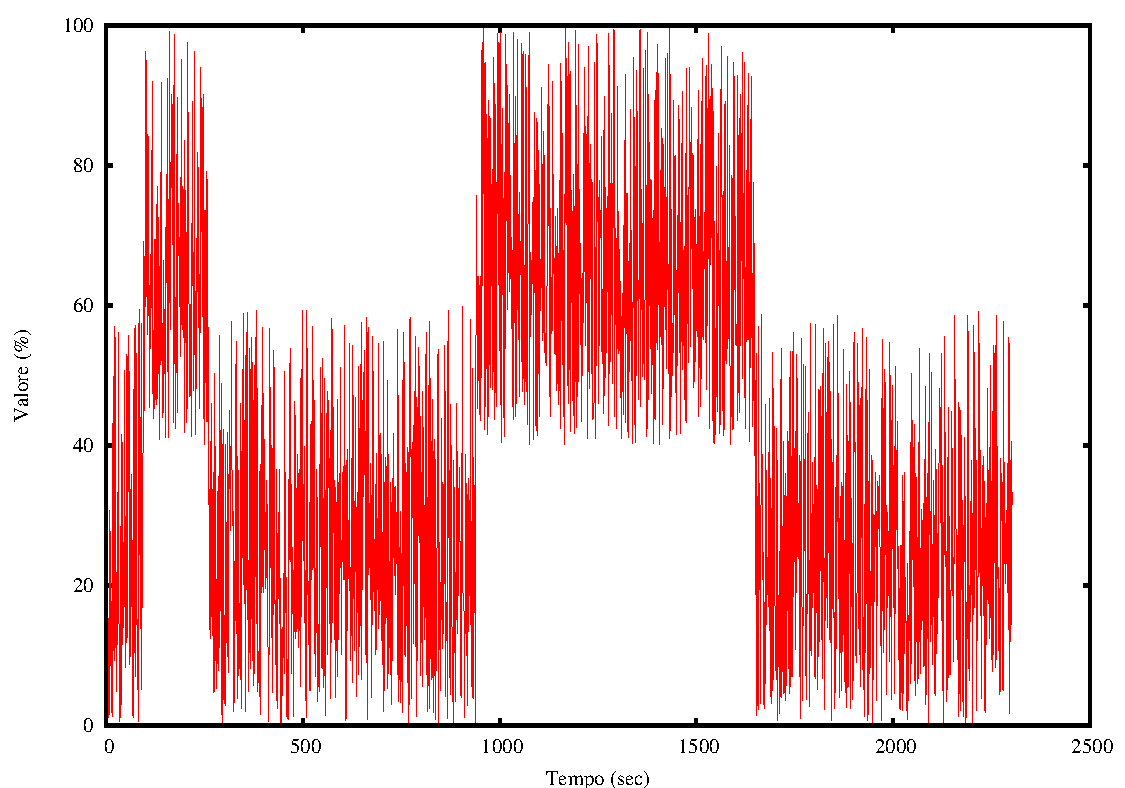
\includegraphics[scale=0.6]{etc/ram3.pdf}
\caption{Ram terzo nodo}
\label{fig:ram3}
\end{center}
\end{figure}
\begin{figure}[H]
\begin{center}
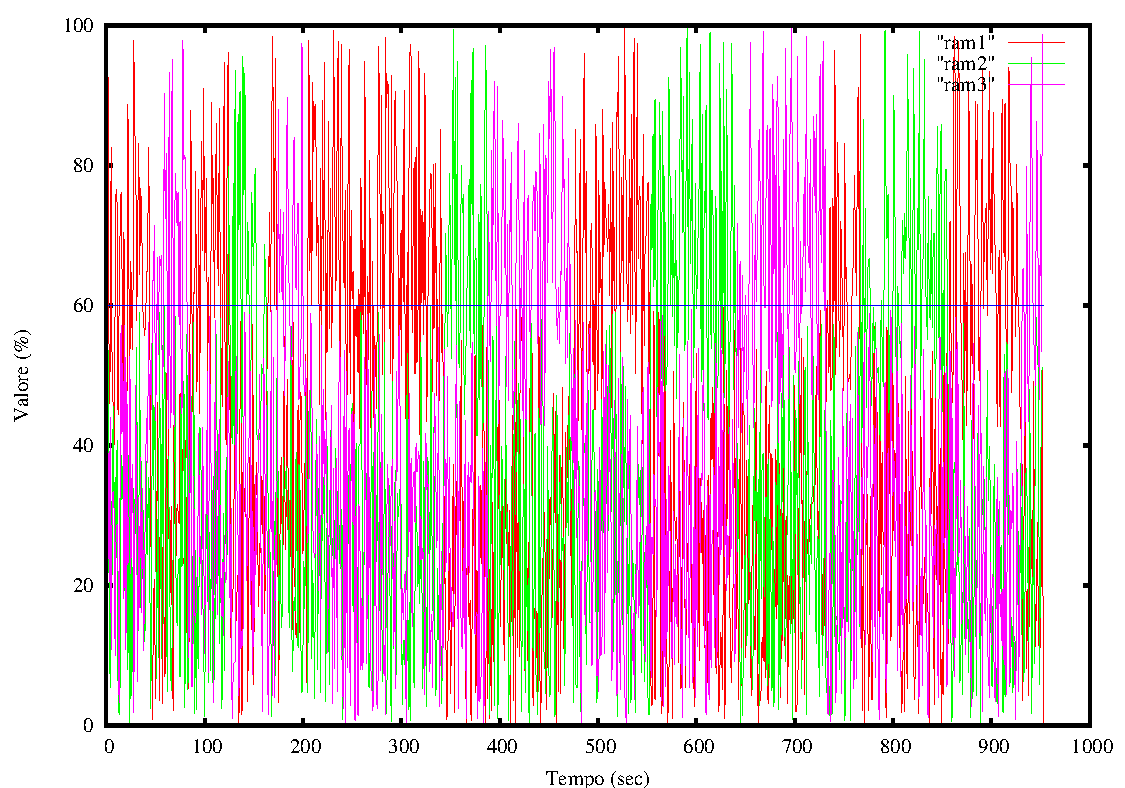
\includegraphics[scale=0.6]{etc/ram.pdf}
\caption{Ram tutti i nodi}
\label{fig:ram}
\end{center}
\end{figure}

\subsection{Memory}
La memoria è un parametro molto più dipendente dalle migrazioni, infatti in corrispondenza di esse si ha un incremento di utilizzazione costante ma non istantaneo. Dai grafici \ref{fig:memory1}, \ref{fig:memory2}, \ref{fig:memory3} e \ref{fig:memory} si può notare che quando i valori di memoria raggiungono la soglia dello 0 o del 100 si ha un picco di traffico verticale, questo non è dovuto alle migrazioni ma potrebbe essere associato, ad esempio, a generazioni di file temporanei da parte del nodo. In corrispondenza di incrementi di memoria costanti vuol dire che è presente lo SC, invece quando si hanno cali costanti si ha il contrario, ovvero lo SC è migrato su un altro nodo.
\begin{figure}[H]
\begin{center}
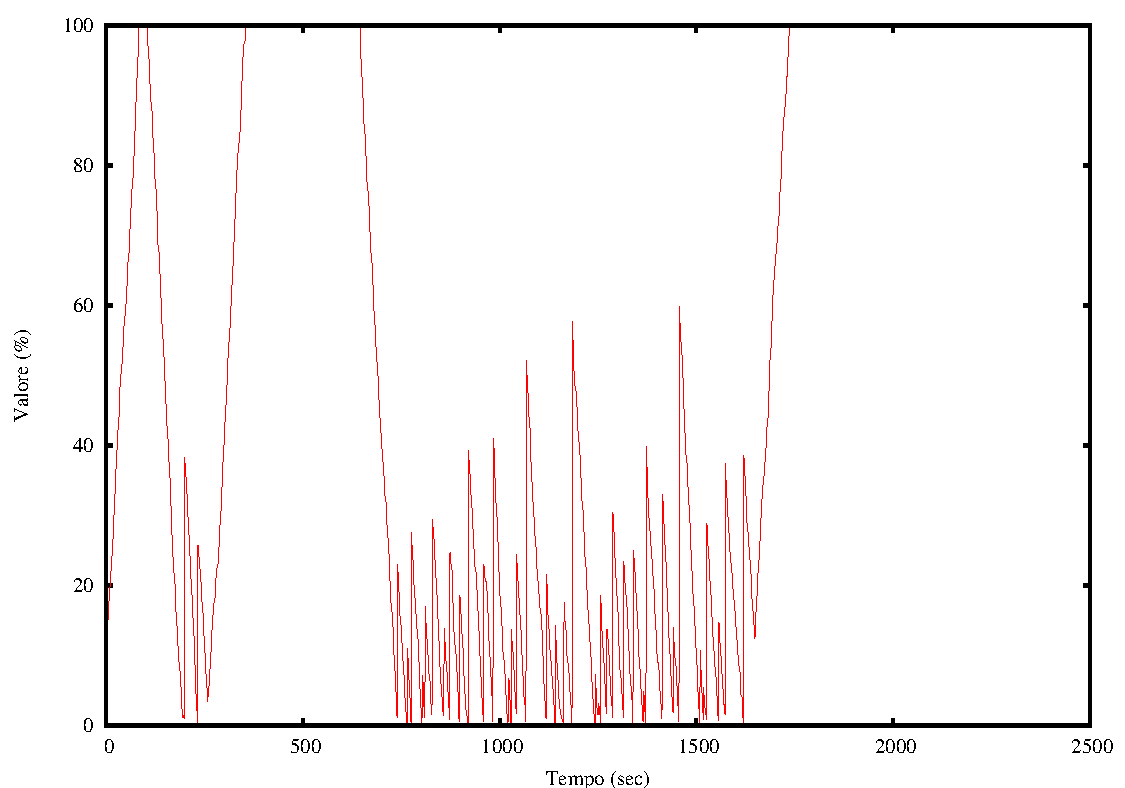
\includegraphics[scale=0.6]{etc/memory1.pdf}
\caption{Memory primo nodo}
\label{fig:memory1}
\end{center}
\end{figure}
\begin{figure}[H]
\begin{center}
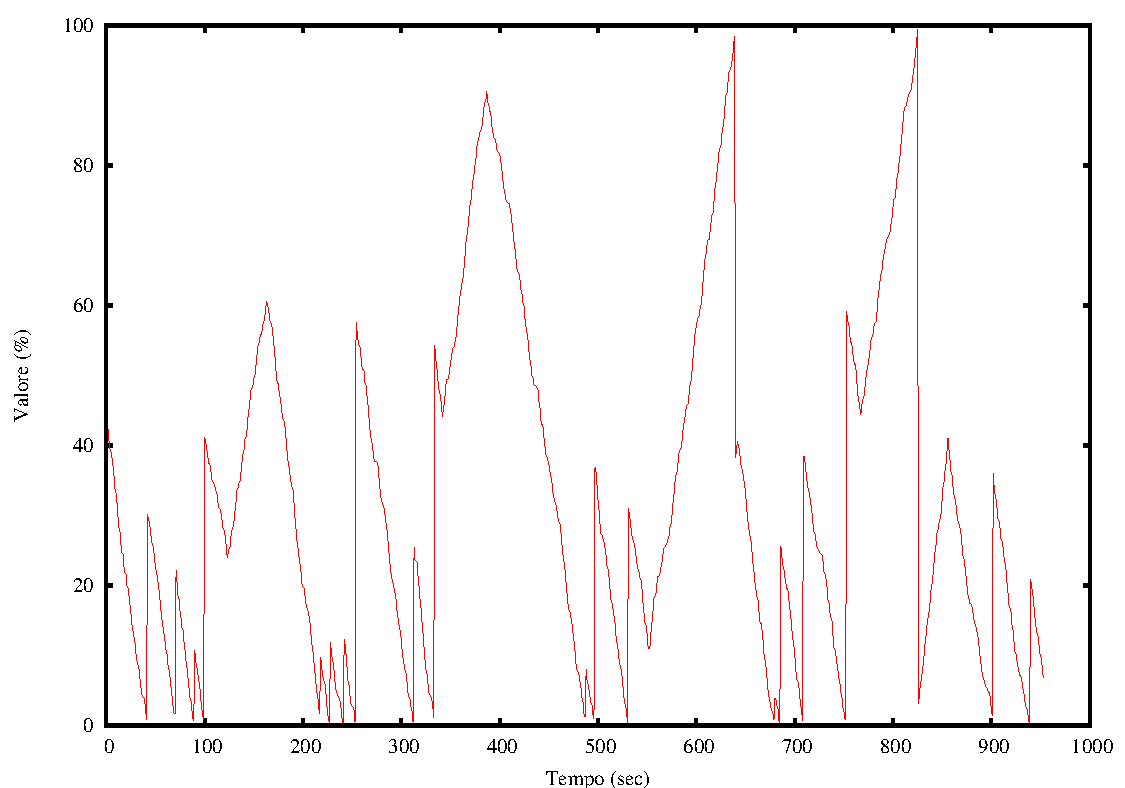
\includegraphics[scale=0.6]{etc/memory2.pdf}
\caption{Memory secondo nodo}
\label{fig:memory2}
\end{center}
\end{figure}
\begin{figure}[H]
\begin{center}
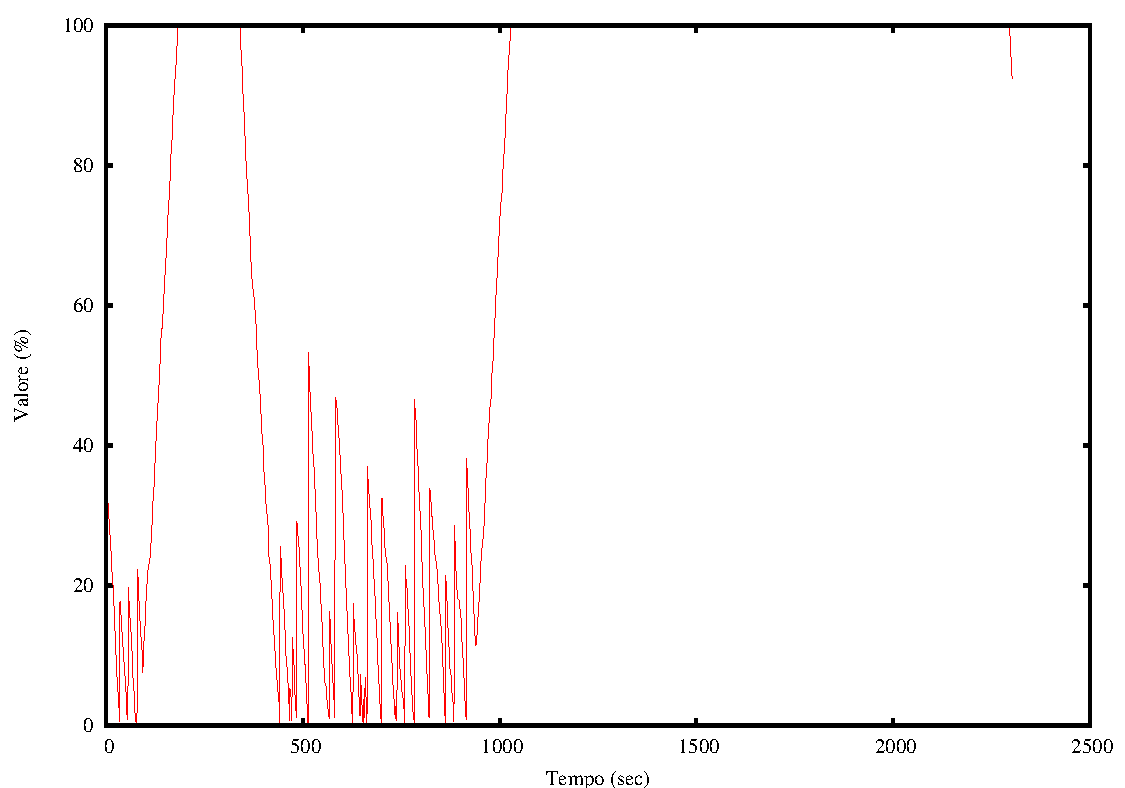
\includegraphics[scale=0.6]{etc/memory3.pdf}
\caption{Memory terzo nodo}
\label{fig:memory3}
\end{center}
\end{figure}
\begin{figure}[H]
\begin{center}
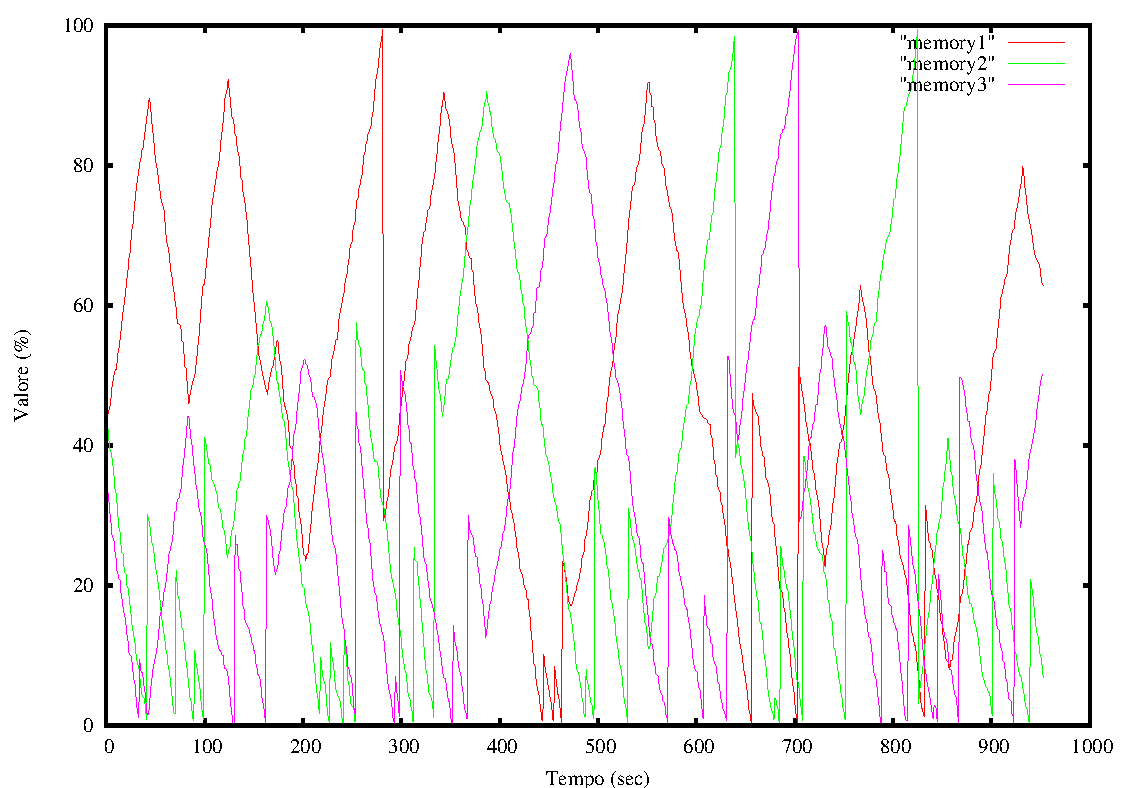
\includegraphics[scale=0.6]{etc/memory.pdf}
\caption{Memory tutti i nodi}
\label{fig:memory}
\end{center}
\end{figure}

\subsection{Energy}
L'energia è il parametro che varia più regolarmente in quanto dipende dal tipo di connessione e dalla presenza delle rete elettrica. Tale comportamento può essere notato dai grafici \ref{fig:energy1}, \ref{fig:energy2}, \ref{fig:energy3} e \ref{fig:energy}. In particolare in presenza dello SC su un nodo si ha un utilizzo di corrente maggiore, nello specifico se il nodo è connesso alla rete elettrica si ha un caricamento più lento, essendo parte dell'energia sprecata a causa dello SC. Anche in caso di scollegamento dalla rete elettrica si ha uno spreco di energia maggiore causato dallo SC, Dalle figure si può anche notare che in corrispondenza del 10\% si ha un incremento di carica, essendo il nodo ricollegato alla rete elettrica, invece al raggiungimento del 100\% viene scollegato, considerando che il caricamento è completo. Un ulteriore particolare si può notare in figura \ref{fig:energy1}, in quanto il nodo è di tipo fisso e quindi con corrente sempre disponibile, infatti il valore di energia è sempre 100\%.
\begin{figure}[H]
\begin{center}
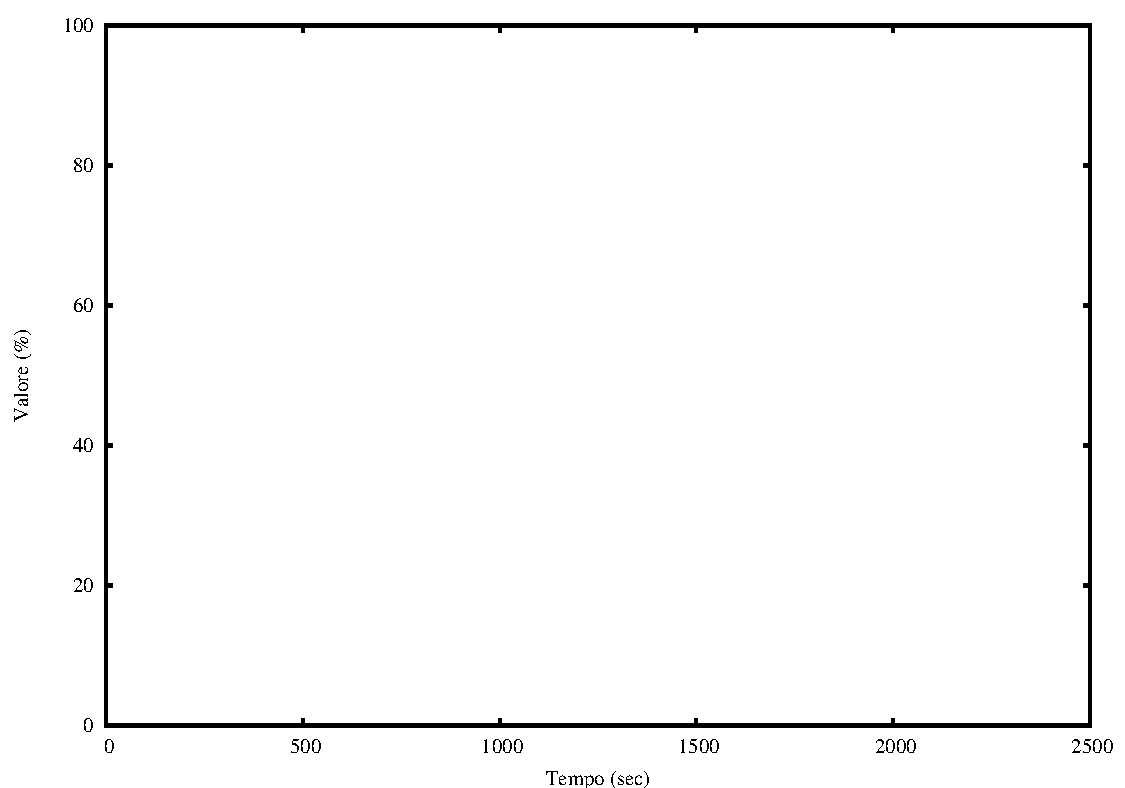
\includegraphics[scale=0.6]{etc/energy1.pdf}
\caption{Energy primo nodo}
\label{fig:energy1}
\end{center}
\end{figure}
\begin{figure}[H]
\begin{center}
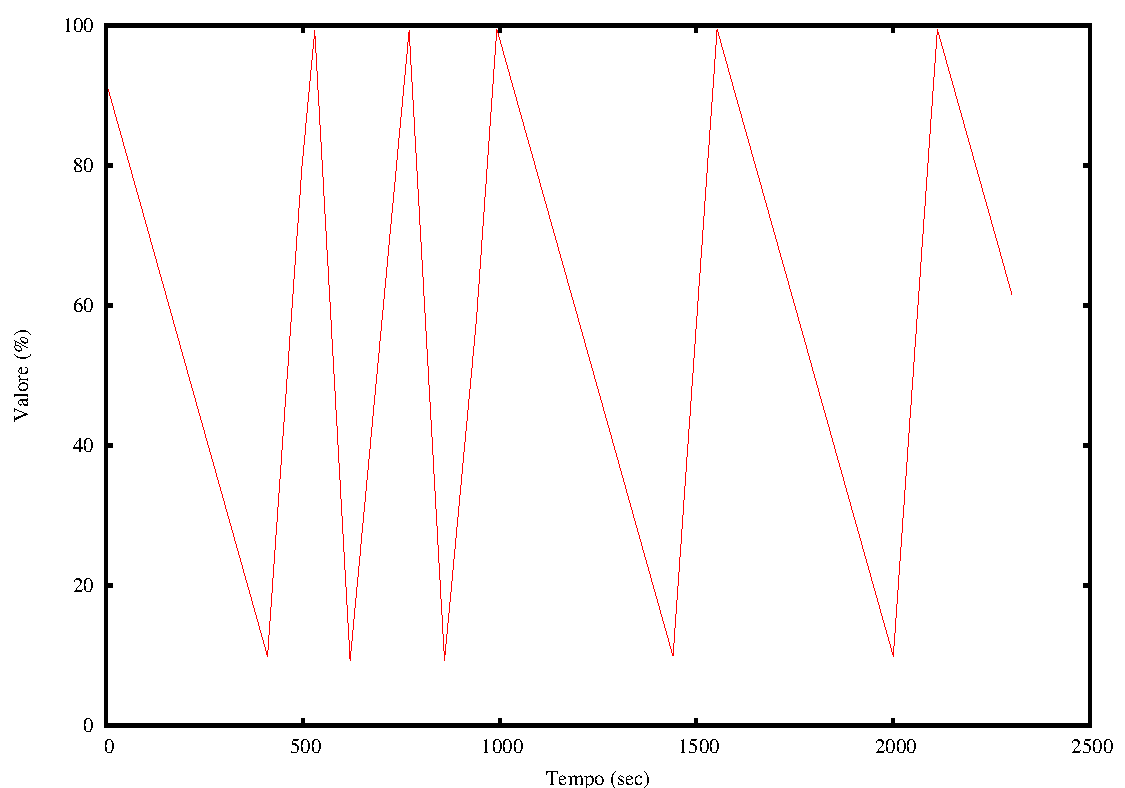
\includegraphics[scale=0.6]{etc/energy2.pdf}
\caption{Energy secondo nodo}
\label{fig:energy2}
\end{center}
\end{figure}
\begin{figure}[H]
\begin{center}
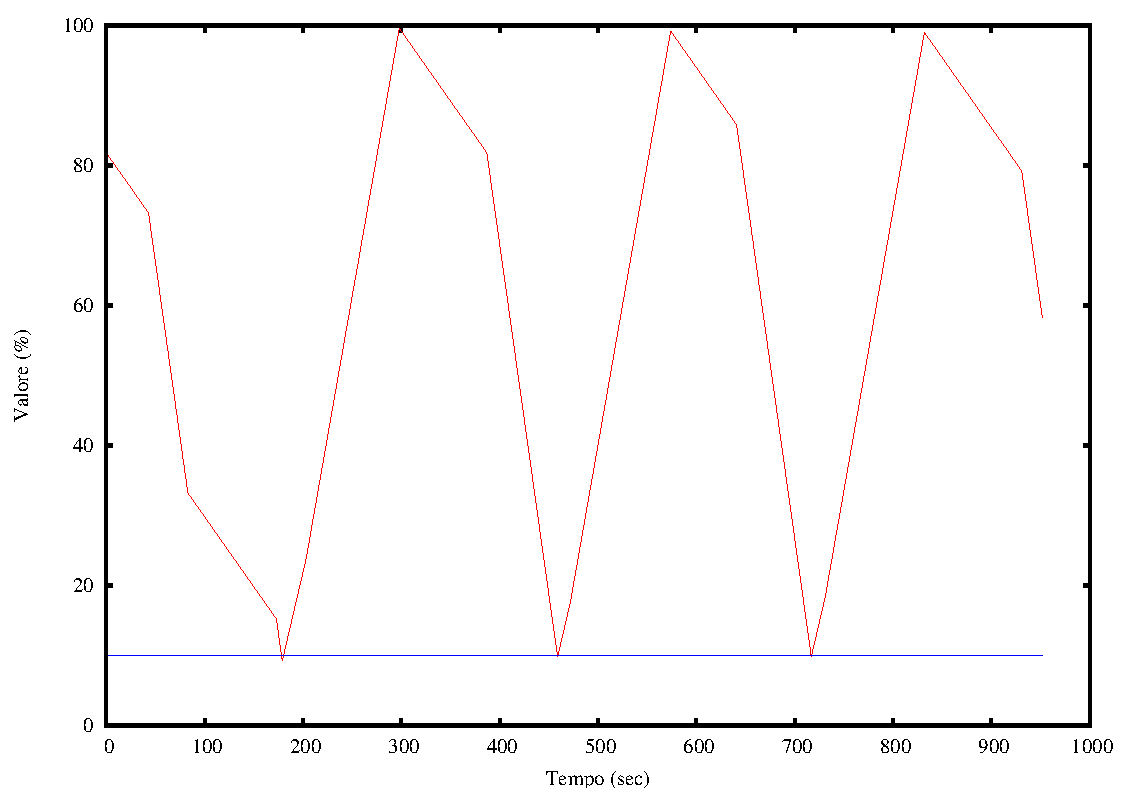
\includegraphics[scale=0.6]{etc/energy3.pdf}
\caption{Energy terzo nodo}
\label{fig:energy3}
\end{center}
\end{figure}
\begin{figure}[H]
\begin{center}
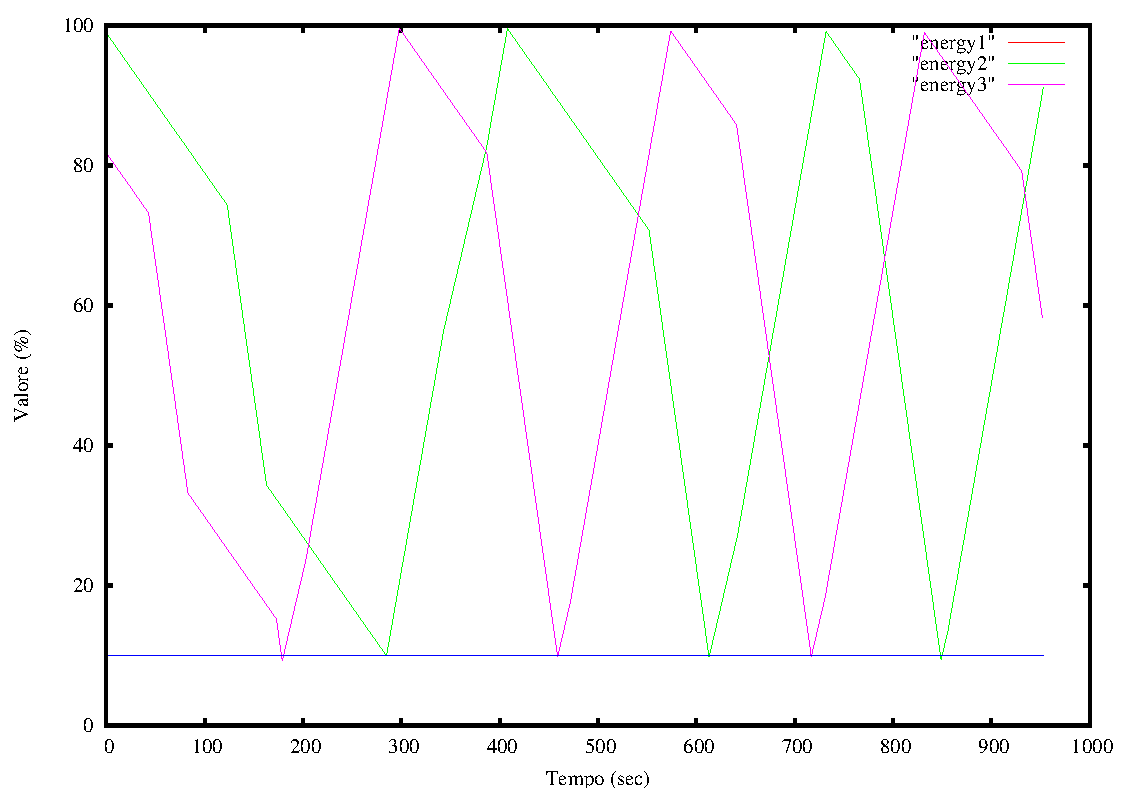
\includegraphics[scale=0.6]{etc/energy.pdf}
\caption{Energy tutti i nodi}
\label{fig:energy}
\end{center}
\end{figure}

\subsection{Latency}
Quest'ultimo valore generato dipendenze dalla presenza dell'SC, dal tipo di linea e dalla banda, come già riportato nel modello matematico. Nei seguenti grafici si possono vedere gli andamenti:
\begin{figure}[H]
\begin{center}
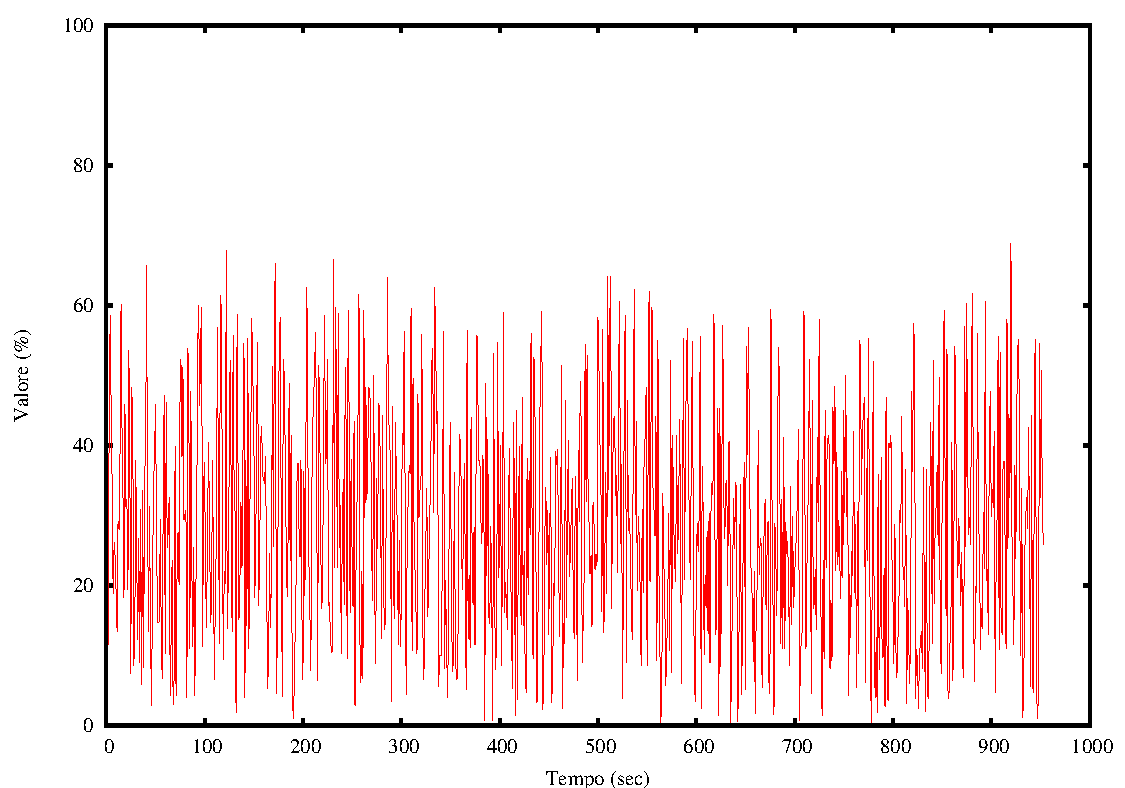
\includegraphics[scale=0.6]{etc/latency1.pdf}
\caption{Latency primo nodo}
\label{fig:latency1}
\end{center}
\end{figure}
\begin{figure}[H]
\begin{center}
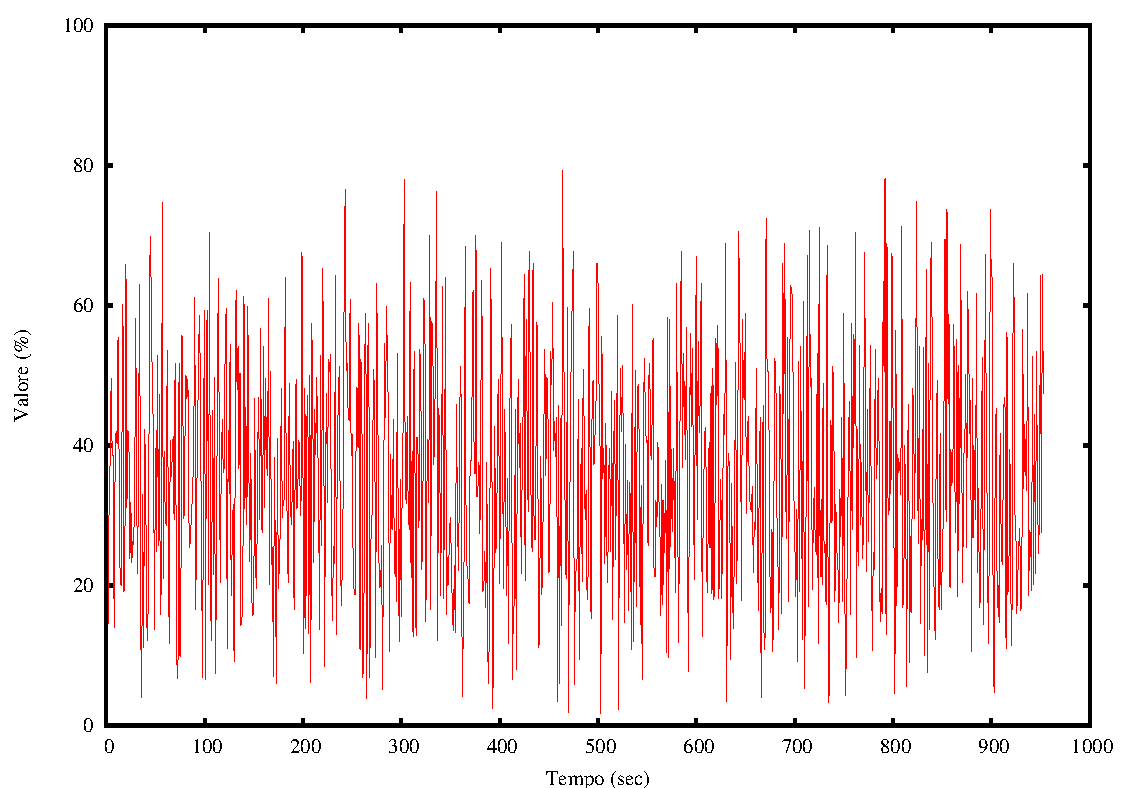
\includegraphics[scale=0.6]{etc/latency2.pdf}
\caption{Latency secondo nodo}
\label{fig:latency2}
\end{center}
\end{figure}
\begin{figure}[H]
\begin{center}
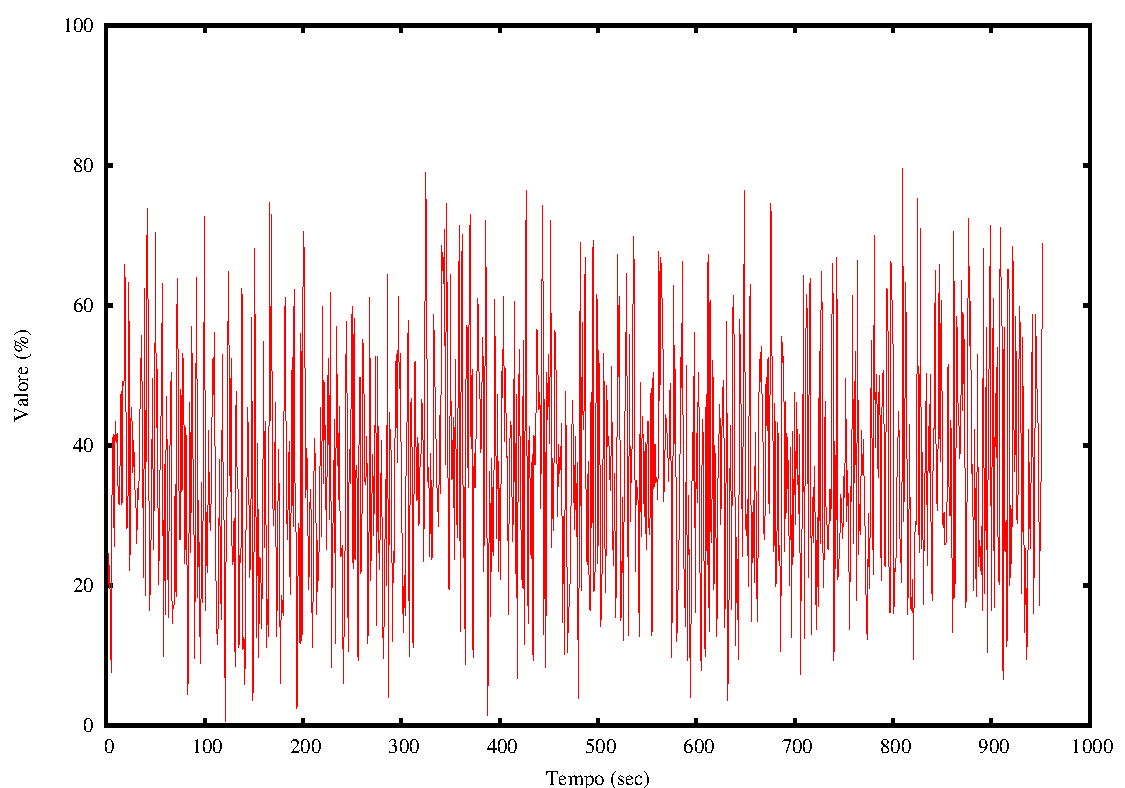
\includegraphics[scale=0.6]{etc/latency3.pdf}
\caption{Latency terzo nodo}
\label{fig:latency3}
\end{center}
\end{figure}
I valori in figura \ref{fig:latency1} è molto più basso rispetto ai valori in figura \ref{fig:latency2} e \ref{fig:latency3}, a causa della tipologia di connessione diversa.

\subsection{Reliability}
Questo valore è simile alla latenza ed anch'esso dipende fortemente dal tipo di connessione e dalla banda ma non dall'SC, il quale non influisce sulle caratteristiche della qualità della connessione. Nelle figure si può notare la differenza di valori tra il caso \ref{fig:reliability1} e i restanti.
\begin{figure}[H]
\begin{center}
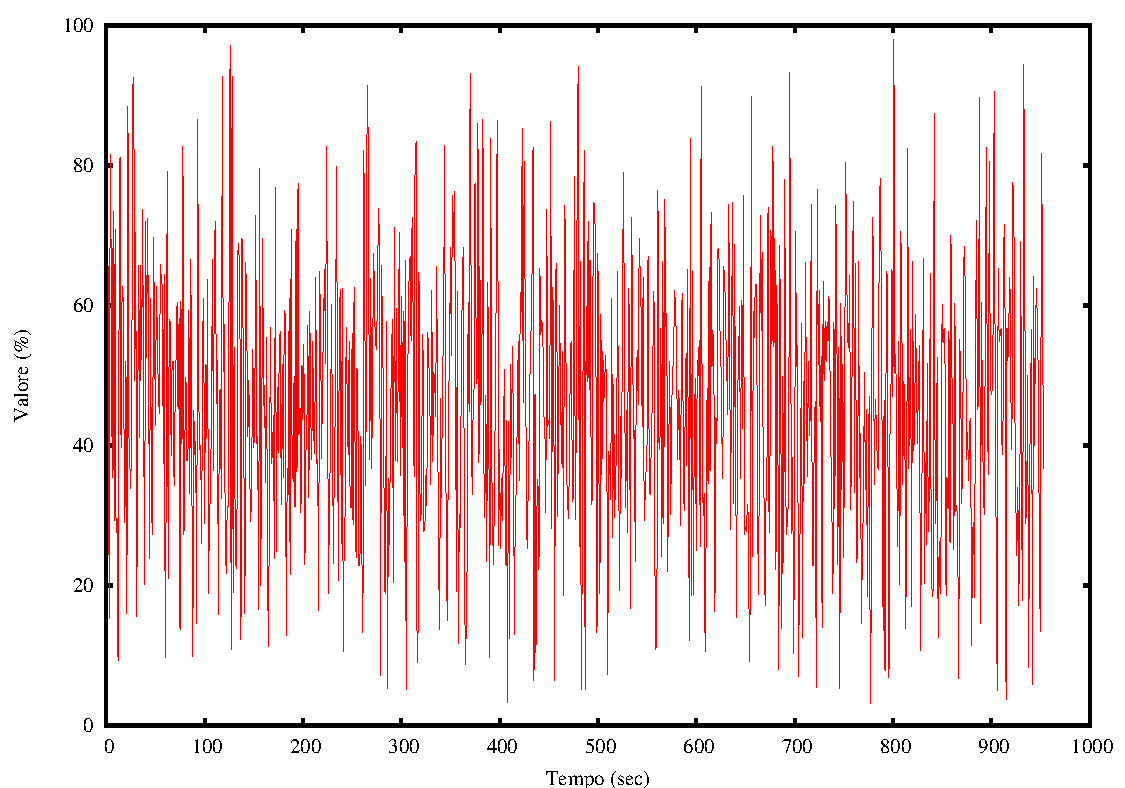
\includegraphics[scale=0.6]{etc/reliability1.pdf}
\caption{Reliability primo nodo}
\label{fig:reliability1}
\end{center}
\end{figure}
\begin{figure}[H]
\begin{center}
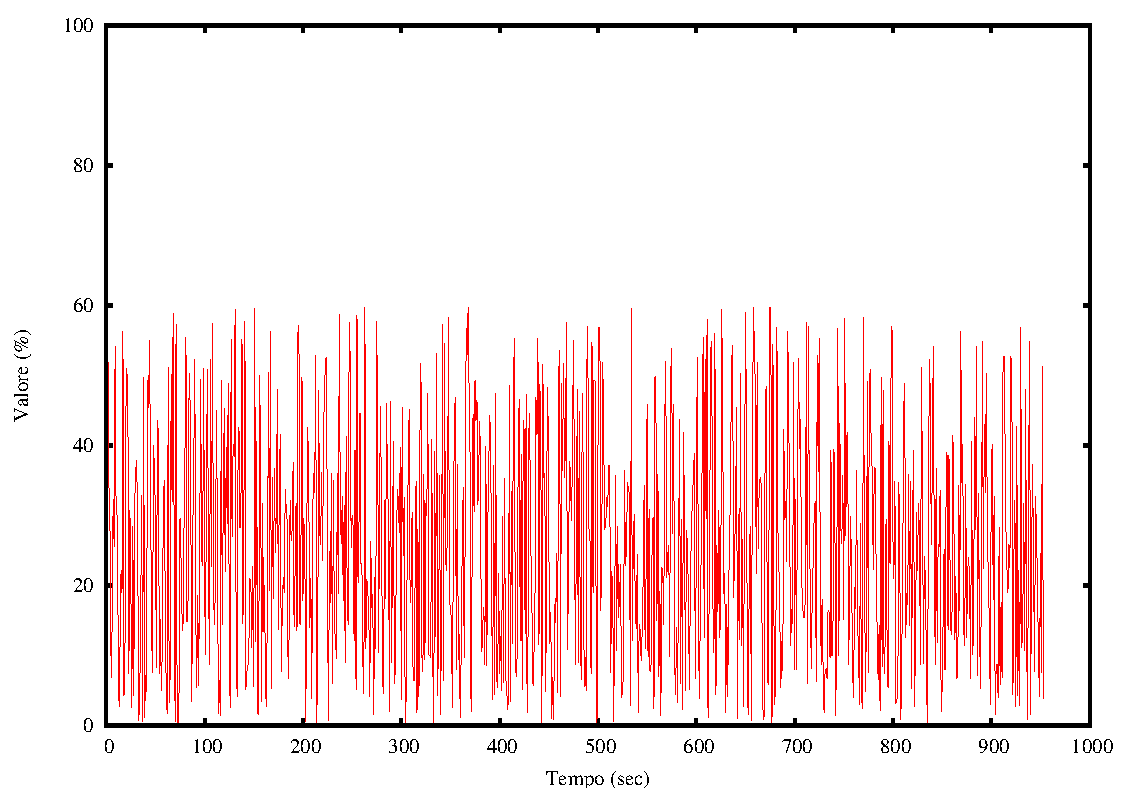
\includegraphics[scale=0.6]{etc/reliability2.pdf}
\caption{Reliability secondo nodo}
\label{fig:reliability2}
\end{center}
\end{figure}
\begin{figure}[H]
\begin{center}
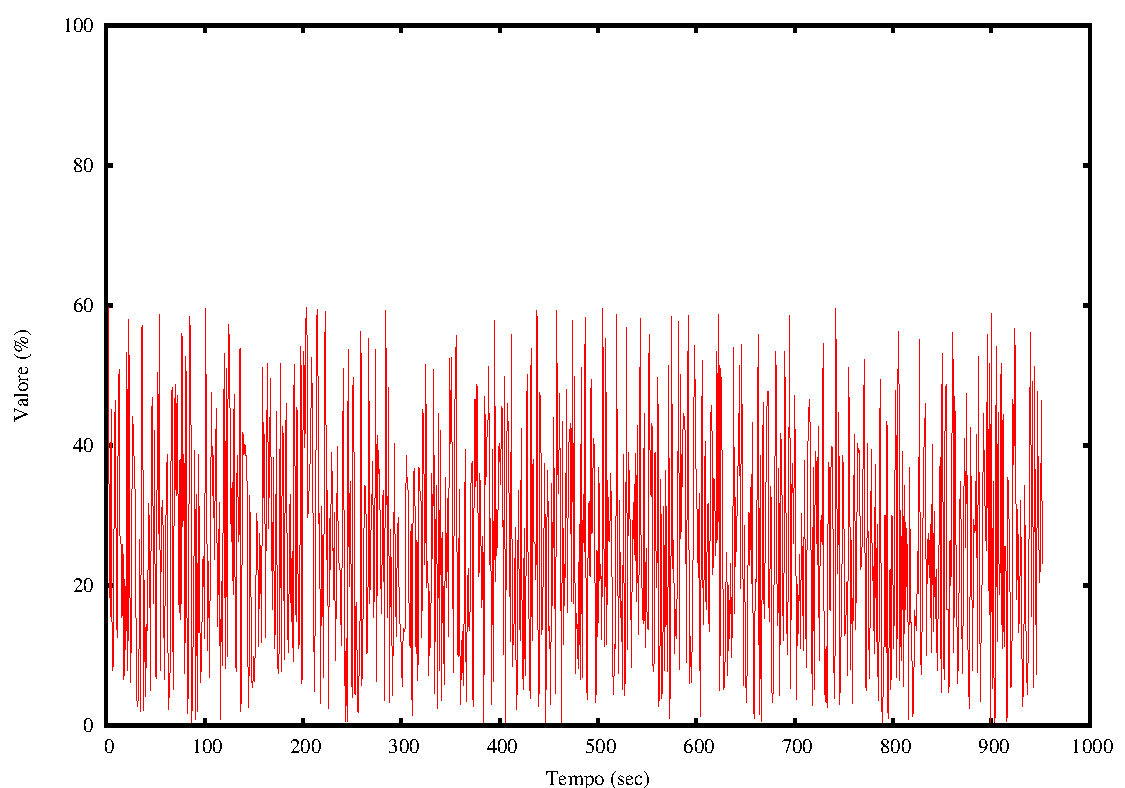
\includegraphics[scale=0.6]{etc/reliability3.pdf}
\caption{Reliability terzo nodo}
\label{fig:reliability3}
\end{center}
\end{figure}

\subsection{ReqInterval}
Quest'ultimo tipo di valore è strettamente casuale e può assumere valori tra lo 0\% e il 100\%.
\chapter{Conclusioni e sviluppi futuri}\label{conclusioni}
E' stato sviluppato un software \textit{P2P} per lo scambio di messaggi tra due o più utenti facendo uso del linguaggio C e delle API del socket di \textit{Berkeley}. Le API dei socket di Berkeley sono state utilizzate per la gestire le connessioni tra peer, permettendo l'instaurazione di connessioni di tipo persistente; inoltre è stato inserito un livello software ex-novo, il quale si comporta come un'interfaccia d'accesso per la comunicazione tra lo strato TCP e quello HTTP su cui si basa l'intero processo di scambio di pacchetti.
I vari test che sono stati eseguiti hanno dimostrato che il sistema riesce a mantenere un buon grado di stabilità e velocità, senza mai trovarsi in uno stato di inconsistenza. Nonostante ciò effettuando un'analisi più dettagliata si possono notare alcune inefficienze, sopratutto per quello che riguarda la gestione dell'invio concorrente dei pacchetti. A tale proposito è stato deciso di adottare un meccanismo di sequenzializzazione dei pacchetti basato sull'utilizzo di particolari strutture come le code e su un algoritmo di polling basato sullo sleep dei \textit{client thread}\index{client thread}.
In questo modo ogni client non rischierà di perdere alcun segnale di notifica, proveniente dal lato server, per l'invio di un pacchetto. Una possibile risoluzione al fine di evitare lo sleeping del thread potrebbe essere l'introduzione di un \texttt{pthread\_cond\_timedwait()}, ovvero una funzione che gestisce la sospensione del thread solo nel caso di ricezione di un segnale o allo scadere del timer. Per quello che riguarda lo sviluppo di funzionalità aggiuntive si potrebbe pensare alla possibilità di effettuare il trasferimento di file tra gli utenti di una chat, funzionalità in parte già sviluppata. Un'ulteriore miglioria all'applicazione potrebbe essere fatta aggiungendo il supporto ad una sorta di \textit{WebCache}\index{WebCache}, ovvero la possibilità di reperire la lista dei peer (necessari al \textit{bootstrap}\index{bootstrap}) da un server centralizzato.
\lstset{backgroundcolor=\color{white}}
\lstset{frame=f}
\chapter{Appendice}\label{appendice}
\section{SLARequesterBehaviour.java}
\lstinputlisting[name=SLARequesterBehaviour.java]{../../src/slash/contextmanager/behaviour/SLARequesterBehaviour.java}

\section{SLAReqReceiverBehaviour.java}
\lstinputlisting[name=SLAReqReceiverBehaviour.java]{../../src/slash/contextmanager/behaviour/SLAReqReceiverBehaviour.java}

\section{ContextProducerBehaviour.java}
\lstinputlisting[name=ContextProducerBehaviour.java]{../../src/slash/contextmanager/behaviour/ContextProducerBehaviour.java}

\section{ViolationConsumerBehaviour.java}
\lstinputlisting[name=ViolationConsumerBehaviour.java]{../../src/slash/contextmanager/behaviour/ViolationConsumerBehaviour.java}

\section{RmConsumerBehaviour.java}
\lstinputlisting[name=RmConsumerBehaviour.java]{../../src/slash/contextmanager/behaviour/RmConsumerBehaviour.java}

\section{ContextManagerAgent.java}
\lstinputlisting[name=ContextManagerAgent.java]{../../src/slash/contextmanager/agent/ContextManagerAgent.java}

\section{CpuResourceBehaviour.java}
\lstinputlisting[name=CpuResourceBehaviour.java]{../../src/slash/resourcemonitor/behaviour/CpuResourceBehaviour.java}

\section{RamResourceBehaviour.java}
\lstinputlisting[name=RamResourceBehaviour.java]{../../src/slash/resourcemonitor/behaviour/RamResourceBehaviour.java}

\section{MemoryResourceBehaviour.java}
\lstinputlisting[name=MemoryResourceBehaviour.java]{../../src/slash/resourcemonitor/behaviour/MemoryResourceBehaviour.java}

\section{EnergyResourceBehaviour.java}
\lstinputlisting[name=EnergyResourceBehaviour.java]{../../src/slash/resourcemonitor/behaviour/EnergyResourceBehaviour.java}

\section{LatencyResourceBehaviour.java}
\lstinputlisting[name=LatencyResourceBehaviour.java]{../../src/slash/resourcemonitor/behaviour/LatencyResourceBehaviour.java}

\section{ReliabilityResourceBehaviour.java}
\lstinputlisting[name=ReliabilityResourceBehaviour.java]{../../src/slash/resourcemonitor/behaviour/ReliabilityResourceBehaviour.java}

\section{ReqIntervalResourceBehaviour.java}
\lstinputlisting[name=ReqIntervalResourceBehaviour.java]{../../src/slash/resourcemonitor/behaviour/ReqIntervalResourceBehaviour.java}

\section{RamRmAgent.java}
\lstinputlisting[name=RamRmAgent.java]{../../src/slash/resourcemonitor/agent/RamRmAgent.java}

\section{MemoryRmAgent.java}
\lstinputlisting[name=MemoryRmAgent.java]{../../src/slash/resourcemonitor/agent/MemoryRmAgent.java}

\section{EnergyRmAgent.java}
\lstinputlisting[name=EnergyRmAgent.java]{../../src/slash/resourcemonitor/agent/EnergyRmAgent.java}

\section{CpuRmAgent.java}
\lstinputlisting[name=CpuRmAgent.java]{../../src/slash/resourcemonitor/agent/CpuRmAgent.java}

\section{LatencyRmAgent.java}
\lstinputlisting[name=LatencyRmAgent.java]{../../src/slash/resourcemonitor/agent/LatencyRmAgent.java}

\section{ReliabilityRmAgent.java}
\lstinputlisting[name=ReliabilityRmAgent.java]{../../src/slash/resourcemonitor/agent/ReliabilityRmAgent.java}

\section{ReqIntervalRmAgent.java}
\lstinputlisting[name=ReqIntervalRmAgent.java]{../../src/slash/resourcemonitor/agent/ReqIntervalRmAgent.java}

\section{AgentLauncher.java}
\lstinputlisting[name=AgentLauncher.java]{../../src/slash/boot/AgentLauncher.java}

\section{SLAReceiverBehaviour.java}
\lstinputlisting[name=SLAReceiverBehaviour.java]{../../src/slash/slachecker/behaviour/SLAReceiverBehaviour.java}

\section{SLACheckerBehaviour.java}
\lstinputlisting[name=SLACheckerBehaviour.java]{../../src/slash/slachecker/behaviour/SLACheckerBehaviour.java}

\section{SLAStarterBehaviour.java}
\lstinputlisting[name=SLAStarterBehaviour.java]{../../src/slash/slachecker/behaviour/SLAStarterBehaviour.java}

\section{ContextConsumerBehaviour.java}
\lstinputlisting[name=ContextConsumerBehaviour.java]{../../src/slash/slachecker/behaviour/ContextConsumerBehaviour.java}

\section{MigrationUtil.java}
\lstinputlisting[name=MigrationUtil.java]{../../src/slash/slachecker/util/MigrationUtil.java}

\section{SLACheckerAgent.java}
\lstinputlisting[name=SLACheckerAgent.java]{../../src/slash/slachecker/agent/SLACheckerAgent.java}

\section{ReqIntervalBehaviour.java}
\lstinputlisting[name=ReqIntervalBehaviour.java]{../../src/slash/resource/behaviour/ReqIntervalBehaviour.java}

\section{NotifyReceiverBehaviour.java}
\lstinputlisting[name=NotifyReceiverBehaviour.java]{../../src/slash/resource/behaviour/NotifyReceiverBehaviour.java}

\section{LatencyBehaviour.java}
\lstinputlisting[name=LatencyBehaviour.java]{../../src/slash/resource/behaviour/LatencyBehaviour.java}

\section{RamBehaviour.java}
\lstinputlisting[name=RamBehaviour.java]{../../src/slash/resource/behaviour/RamBehaviour.java}

\section{CpuBehaviour.java}
\lstinputlisting[name=CpuBehaviour.java]{../../src/slash/resource/behaviour/CpuBehaviour.java}

\section{MemoryBehaviour.java}
\lstinputlisting[name=MemoryBehaviour.java]{../../src/slash/resource/behaviour/MemoryBehaviour.java}

\section{EnergyBehaviour.java}
\lstinputlisting[name=EnergyBehaviour.java]{../../src/slash/resource/behaviour/EnergyBehaviour.java}

\section{ReliabilityBehaviour.java}
\lstinputlisting[name=ReliabilityBehaviour.java]{../../src/slash/resource/behaviour/ReliabilityBehaviour.java}

\section{CpuAgent.java}
\lstinputlisting[name=CpuAgent.java]{../../src/slash/resource/agent/CpuAgent.java}

\section{ResourceAgent.java}
\lstinputlisting[name=ResourceAgent.java]{../../src/slash/resource/agent/ResourceAgent.java}

\section{MemoryAgent.java}
\lstinputlisting[name=MemoryAgent.java]{../../src/slash/resource/agent/MemoryAgent.java}

\section{EnergyAgent.java}
\lstinputlisting[name=EnergyAgent.java]{../../src/slash/resource/agent/EnergyAgent.java}

\section{ReliabilityAgent.java}
\lstinputlisting[name=ReliabilityAgent.java]{../../src/slash/resource/agent/ReliabilityAgent.java}

\section{ReqIntervalAgent.java}
\lstinputlisting[name=ReqIntervalAgent.java]{../../src/slash/resource/agent/ReqIntervalAgent.java}

\section{LatencyAgent.java}
\lstinputlisting[name=LatencyAgent.java]{../../src/slash/resource/agent/LatencyAgent.java}

\section{RamAgent.java}
\lstinputlisting[name=RamAgent.java]{../../src/slash/resource/agent/RamAgent.java}

\section{DFUtil.java}
\lstinputlisting[name=DFUtil.java]{../../src/slash/df/DFUtil.java}

\section{Context.java}
\lstinputlisting[name=Context.java]{../../src/slash/entity/Context.java}

\section{Notify.java}
\lstinputlisting[name=Notify.java]{../../src/slash/entity/Notify.java}

\section{SLAContract.java}
\lstinputlisting[name=SLAContract.java]{../../src/slash/entity/SLAContract.java}

\section{DataWriter.java}
\lstinputlisting[name=DataWriter.java]{../../src/slash/util/DataWriter.java}

\section{PropertiesReader.java}
\lstinputlisting[name=PropertiesReader.java]{../../src/slash/util/PropertiesReader.java}

\section{DsmServerBehaviour.java}
\lstinputlisting[name=DsmServerBehaviour.java]{../../src/slash/dsm/behaviour/DsmServerBehaviour.java}

\section{DsmDataManager.java}
\lstinputlisting[name=DsmDataManager.java]{../../src/slash/dsm/data/DsmDataManager.java}

\section{Tuple.java}
\lstinputlisting[name=Tuple.java]{../../src/slash/dsm/tuple/Tuple.java}

\section{DsmServerAgent.java}
\lstinputlisting[name=DsmServerAgent.java]{../../src/slash/dsm/agent/DsmServerAgent.java}

\section{DsmClient.java}
\lstinputlisting[name=DsmClient.java]{../../src/slash/dsm/client/DsmClient.java}


\lstlistoflistings
\listoftables
\listoffigures
\printindex
\bibliographystyle{plain}
\bibliography{cap/bibliografia}

\end{document}